\RequirePackage{etex}
\documentclass[10pt, superscriptaddress,aps,pra,twocolumn,showpacs,nofootinbib, longbibliography, notitlepage,floatfix]{revtex4-2}
% \usepackage[utf8]{inputenc}
\usepackage[utf8]{inputenc}
\usepackage[T1]{fontenc}
\usepackage{etex}
\usepackage{amsmath,amssymb,amsthm}
\usepackage[colorlinks=true,citecolor=blue,urlcolor=blue]{hyperref}
\usepackage[pdftex]{graphicx}
\usepackage{times,txfonts}
\usepackage{braket}
\usepackage{color}
\usepackage{natbib}
\usepackage{amsmath,blkarray}
\usepackage{mathtools}
\usepackage{ulem}
\usepackage{latexsym}
\usepackage{tabularx, booktabs}
\usepackage{graphics,epstopdf}
\usepackage{graphicx}
% \usepackage{float}
\usepackage{amsfonts}
\usepackage{MnSymbol,graphicx}
 % \usepackage[utf8]{inputenc}

\newtheorem{theorem}{Theorem}

\usepackage{amsthm}
\newtheorem{proposition}{Proposition}
 
\usepackage{natbib}

\newcommand{\ka}[1]{{\color{violet}#1}}

% \usepackage{algorithm}
% \usepackage{algorithmic}
\usepackage{indentfirst}


\usepackage{tikz}
\usetikzlibrary{shapes,arrows,positioning}


% \let\algorithm\relax
\usepackage[ruled]{algorithm2e}
\usetikzlibrary{quantikz2}
\usepackage{color,soul}
\newcommand{\blu}{\color{blue}}
\newcommand{\grn}{\color{green}}
\newcommand{\red}{\color{red}}
\newcommand{\blue}{\color{blue}}
%\newcommand{}{\color{red}}
\newcommand{\be}{\begin{equation}}
\newcommand{\ee}{\end{equation}}
\newcommand{\ba}{\begin{eqnarray}}
\newcommand{\ea}{\end{eqnarray}}
\newcommand{\ketbra}[2]{|#1\rangle \langle #2|}
\newcommand{\tr}{\operatorname{Tr}}
\newcommand{\one}{\bf{1}}
\newcommand{\half}{\frac{1}{2}}
\newcommand{\qua}{\frac{1}{4}}
\newcommand{\etal}{{\it{et al. }}}
\newcommand{\plane}[2]{$#1#2$\nobreakdash-plane}
\newtheorem{cor}{Corollary}
\newtheorem{observation}{Observation}
\newtheorem{definition}{Definition}
% \newtheorem{proposition}{Proposition}
\newtheorem{example}{Example}
\newtheorem{thm}{Theorem}
\usepackage{multirow}
\usepackage{appendix}
\usepackage{url}
\usepackage{orcidlink}
\renewcommand{\arraystretch}{1.7}
\newtheorem{Lemma}{Lemma}
\newtheorem{remark}{Remark}
\newtheorem{scenario}{Scenario}
\def \hfillx {\hspace*{-\textwidth} \hfill}
\renewcommand{\bibsection}{}   
% \renewcommand{\abstractname}{Abstract}

\input{shortcut.tex}

\begin{document}
\title{{Noise-Assisted Feedback Control of Open Quantum Systems for Ground State Properties}}

\author{Kasturi Ranjan Swain}
\email{{kasturi.swain@uni.lu}}
\affiliation{Department  of  Physics  and  Materials  Science,  University  of  Luxembourg,  L-1511  Luxembourg,  Luxembourg}
\author{Rajesh K. Malla}
\email{{malla@aps.org}}
\affiliation{Physical Review Letters, American Physical Society, Hauppauge, New York 11788, USA}
\affiliation{Condensed Matter Physics and Materials Science Division, Brookhaven National Laboratory, Upton, New York 11973, USA}
\author{Adolfo del Campo}                 
\affiliation{Department  of  Physics  and  Materials  Science,  University  of  Luxembourg,  L-1511  Luxembourg,  Luxembourg}
\affiliation{Donostia International Physics Center,  E-20018 San Sebasti\'an, Spain}

\begin{abstract}
Intrinsic noise in pre-fault-tolerant quantum devices poses a major challenge to the reliable realization of unitary dynamics in quantum algorithms and simulations. To address this, we present a method for simulating open quantum system dynamics on a quantum computer, including negative dissipation rates in the Gorini-Kossakowski-Sudarshan-Lindblad (GKSL) master equation. Our approach lies beyond the standard Markovian approximation, enabling the controlled study of non-Markovian processes within a quantum simulation framework. Using this method, we develop a quantum algorithm for calculating ground-state properties that exploits feedback-controlled, noise-assisted dynamics. In this scheme, Lyapunov-based feedback steers the system toward a target virtual state under engineered noise conditions. While noisy simulations typically fail to converge and degrade in performance as noise accumulates over time, our method exhibits improved convergence, albeit with an increased exponential sampling overhead. This framework offers a promising strategy for harnessing current quantum hardware and advancing robust control protocols based on open-system dynamics.
\end{abstract}
\maketitle 

\section*{Introduction}
Digital quantum simulation (DQS) provides a promising pathway for simulating quantum many-body systems using state-of-the-art quantum computers~\cite{Arute2019, Pan_PRL_2021}. However, inherent noise in quantum devices remains a significant obstacle to performing meaningful computations, especially when aiming to demonstrate a quantum advantage over classical computers. Pre-fault-tolerant quantum devices commonly experience dissipation, decay, and decoherence, significantly limiting the circuit depth and the manageable system size~\cite{Bharti_RevModPhys_2022}. In parallel with hardware advances that reduce environmental effects, extensive efforts are underway to address noise through quantum error mitigation~\cite{Cai_QEM_2023}, quantum error correction~\cite{PhysRevA_surface_code}, and noise suppression methods. Ongoing theoretical and experimental advances are jointly driving progress toward realizing quantum advantage.

DQS in quantum devices typically requires Trotterization of the system dynamics into native quantum gates. However, due to intrinsic noise, the dynamics of closed systems realized in actual quantum hardware often resemble that of open quantum systems (OQS). Several theoretical and experimental studies have proposed harnessing noise as a resource for various applications, including thermal and ground-state preparation~\cite{Terhal_pra_2000, kraus_pra_2008, Verstraete2009, Kapit_2017, science_dissipation}, quantum information processing~\cite{Harrington2022_nat_phys}, and simulation of open quantum systems~\cite{PhysRevA.108.062424, Pleino_PRX_2023}. Such efforts are crucial, as error correction generally incurs substantial overhead in physical qubits and gates, making its practical implementation challenging~\cite{PhysRevA_surface_code}.

To simulate open quantum systems, rather than conventional isolated many-body systems, a variety of strategies have been proposed ~\cite{Nori_pra_2011, Solano_Pra_2016, PRXQuantum.5.020332, Delgado_Granados2025}, including simulating the Lindblad master equation via imaginary-time evolution~\cite{PRXQuantum_Motta_2022}, the Kraus operator formalism~\cite{Hu2020, Mazziotti_PRL_2021}, Trotterization methods~\cite{PhysRevLett.127.020504}, and variational algorithms~\cite{PRR_VQE_NESS_2020_Fujii, 2020_prl_Endo}. However, these methods often face scalability challenges due to the need for ancillary qubits or mid-circuit measurements. As a result, stochastic approaches present a systematic solution to overcome scalability limitations~\cite{Aurelia_adc_2017, Narang_PRR_2021, peng2024quantumtrajectoryinspiredlindbladiansimulation, Sandro_Donadi_PRR_2024, borras2024quantumalgorithmsimulatelindblad, liu2024simulationopenquantumsystems, huang2025robustvariationalquantumsimulation}. Furthermore, accurately modeling environmental noise often entails information flow from the environment back into the system, thereby violating the Markovian approximation. The framework of non-Markovian open quantum systems thus offers a more realistic description and deeper insight into dissipation and decoherence processes~\cite{Zoller_book_noise}. Therefore, algorithms that incorporate non-Markovian dynamics are central to the realistic simulation of open quantum systems ~\cite{Modi_PRXQuantum_2021, trivdei_cirac_2025_arxiv, cai_non_markov_2025}.

{Here we propose a method to simulate a class of non-Markovian time-dependent dynamics of an OQS in a digitized quantum circuit. By non-Markovian, we specifically refer to dynamics governed by a time-local Gorini–Kossakowski–Sudarshan–Lindblad (GKSL)  master equation with negative decay rates~\cite{Breuer_book}, a regime that, while formally unphysical as a standalone noise channel, can be implemented via classical post-processing through the pseudo-Lindblad quantum trajectory (PLQT)~\cite{Eckardt_PRL} or the quasiprobability decomposition (QPD) methods~\cite{Gambetta2017PRL, Cai_QEM_2023}. Importantly, such negative rates are not merely a theoretical construction; recent independent works demonstrate that they arise generically in noisy intermediate-scale quantum (NISQ) devices under Pauli twirling, corroborating the physical regime in which our algorithm operates~\cite{kattemolle2026_arxiv, seif2026_arxiv}.}

With the PLQT approach, an arbitrary noisy process in Lindblad form can be implemented on an ideal quantum circuit using any quantum computing software development kit, such as the AerSimulator of Qiskit~\cite{Qiskit2021}. However, in the quantum trajectory approach, the system evolves through pure states, a condition that is generally unattainable in experiments. For experimental implementation, we demonstrate a method that uses noise as a resource to simulate non-Markovian time-dependent dynamics, leveraging quantum error mitigation techniques such as the QPD method. A critical step in our algorithm is to characterize intrinsic noise in each circuit layer using randomized compiling and cycle error reconstruction methods~\cite{EmersonPRA2016, Flammia2020, EmersonPRX2021}. Error mitigation protocols allow one to compute the expectation values of quantum observables and may provide a path toward the quantum advantage~\cite{Blatt_nat_comm_2019, vandenBerg2023_natphys, Kim2023, aharonov2025importanceerrormitigationquantum, zimborás2025mythsquantumcomputationfault}. The motivation of this work aligns with that of improving the capabilities of near-term quantum hardware to perform useful tasks. 

We integrate our scheme to simulate non-Markovian OQS dynamics with feedback-based quantum algorithms (FQAs), introducing the noise-assisted feedback-based quantum algorithm (NAFQA). FQAs were originally proposed to find solutions to combinatorial optimization problems~\cite{SarovarPRL2022, Magann_PRA_2022}, with broad applications in industry and academia, ranging from job-shop scheduling to drug discovery. However, experimental implementations often fail to find optimal solutions due to the intrinsic noise of the device~\cite{SarovarPRL2022, RKMalla_PRR_2024}. {Rather than treating the (non-Markovian) noise as a nuisance to be suppressed, we propose to exploit it as a feedback-controlled computational resource, using Lyapunov-based control to engineer the negative rates layer-by-layer to enforce monotone energy descent. Unlike passive dissipative cooling protocols, in which Lindblad operators and decay rates are fixed a priori to engineer a target steady state~\cite{Verstraete2009, kraus_pra_2008, science_dissipation}, NAFQA employs a closed-loop, feedback-adaptive strategy that operates directly on the native noise of the device; a detailed comparison with dissipative and variational approaches is presented in the Discussion.} 

We apply NAFQA to the max-cut and spin-glass problem Hamiltonians. Our results demonstrate that feedback-based OQS dynamics with intrinsic noise converges more rapidly to the virtual ground state than closed-system dynamics, as the presence of noise enforces a negative energy gradient at each step, thereby accelerating population transfer to virtual low-energy states. As with other error mitigation strategies, our approach incurs an exponential overhead in certain parameters~\cite{Takagi2022}. Its applicability is limited to physical scenarios with a low number of decay channels and does not constitute an alternative to quantum error correction. Although we primarily focus on the DQS here, our approach is not limited to gate-based quantum computers and can also be realized in analog settings. The QPD assumes a simplified noise channel, modeled either before or after the Trotterized layer of a quantum circuit. In contrast, analog simulations do not need discretization, and our non-Markovian dynamics protocol can be realized with continuous pulses of recovery operations~\cite{Jinzhao_Sun_PhysRevApplied_2021}. Our approach may also find applications in error correction, particularly in autonomous quantum error correction, where dissipation helps stabilize trapped-ion qubits~\cite{Reiter_Zoller_nat_comm_2017}.

\section*{Results}
Our protocol follows a two-step approach. The first step aims to characterize and control the noise associated with each layer by constructing a noise map that integrates noise characterization techniques with the PLQT or the QPD method. In the second step, we introduce feedback-based control parameters using quantum Lyapunov control to {accelerate population transfer toward the virtual many-body ground states}. We emphasize that our approach enables the determination of ground-state properties—such as short- and long-range correlators, dipole moments, and related observables—at the end of the protocol, rather than the true ground state itself.

\subsection*{Non-Markovian dynamics}
The implementation of quantum circuits in DQS inherently involves noise, which can arise from various sources, such as cross-talk, dephasing, energy relaxation, charge noise, etc. To learn the noise, the errors can first be converted to stochastic Pauli errors by randomly applying Paulis before and after noisy gates with a technique known as randomized compiling or Pauli twirling~\cite{EmersonPRA2016, EmersonPRX2021}. Then, the noise associated with each layer of the ideal unitary operator $U$ can be modeled by introducing a stochastic Pauli noise map $\Lambda$ along with the ideal map $\mathcal{U}$. The calligraphic symbol $\mathcal{U}$ denotes a quantum channel corresponding to a unitary $U$ and its action on the density matrix is defined as $\mathcal{U}: \rho \rightarrow U \rho U^{\dagger}$, where $U$ consists of single- and two-qubit Clifford gates. The stochastic noise map $\Lambda$ corresponds to a mixed unitary quantum channel and is expressed as 
\begin{equation}
    \rho \rightarrow \Lambda(\rho) = \sum_{P \in \{I,X,Y,Z\}^{\otimes N}} \lambda_P P \rho P^{\dagger},\label{gen_pauli_channel}
\end{equation}
where $I, X, Y, Z$ denotes the Pauli matrices, and $\lambda_P$ is the relative error probability associated with the Pauli string $P$ that satisfies the condition $\sum_P \lambda_P = 1$. These error probabilities $\{ \lambda \}$ of NISQ devices can be learned efficiently, as demonstrated in recent experiments~\cite{Blatt_nat_comm_2019, vandenBerg2023_natphys, Kim2023, fischer2024dynamicalsimulationsmanybodyquantum}.

Once the noise is learned, we add an additional noise map $\Lambda_s'$ via the PLQT or the QPD method~\cite{Eckardt_PRL, Gambetta2017PRL}. Here, we use the subscript `$s$' for the $s^{\text{th}}$ Trotter step. The combination of these maps simulates effective non-Markovian, time-dependent dynamics, depicted as
\begin{equation}
% \centering
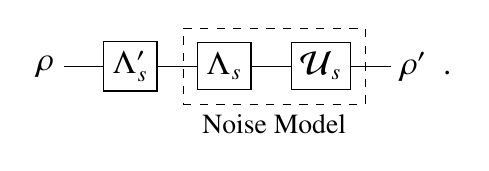
\begin{tikzpicture}
    % Define nodes
    \node (rho) {\large $\rho$};
    \node[draw, minimum size=6mm, right=0.5cm of rho] (E1) {\large $\Lambda_s'$};
    \node[draw, minimum size=6mm, right=0.5cm of E1] (G) {\large $\Lambda_s$};
    \node[draw, minimum size=6mm, right=0.5cm of G] (E2) {\large $\mathcal{U}_s$};
    \node[right=0.5cm of E2] (rho') {\large $\rho'$ ~.};

    % Draw lines
    \draw[-] (rho) -- (E1);
    \draw[-] (E1) -- (G);
    \draw[-] (G) -- (E2);
    \draw[-] (E2) -- (rho');

    \node[draw, dashed, fit=(G) (E2), inner sep=5pt] (box) {};
    \node[below=0pt of box] {Noise Model};\label{non_Markovian-ckt}
\end{tikzpicture}
\end{equation}
The resulting noisy operation $\mathcal {F}_s = \Lambda_s \circ \Lambda_s'$,  with `$\circ$' denoting the composition of maps,  captures the targeted non-Markovian dynamics, which can be associated with the GKSL master equation~\cite{Breuer_book} with negative decay rates. Note that Eq.~\eqref{non_Markovian-ckt} can be expressed as {$\rho(t+ dt) = \mathcal{{U}}_s \mathcal {F}_s (\rho(t))$}, where the superopertaor $\mathcal {F}_s$ represents the noisy dynamics for a small time interval of $dt$. Our method can be understood as coupling the noise source of NISQ devices to an additional bath, with the resulting combined effect treated as a resource for quantum computation. 

We emphasize that although negative error rates correspond to unphysical noisy channels, they can be incorporated into the quantum circuit via techniques such as PLQT or the QPD approach, with appropriate classical post-processing~\cite{Donvil2022, Eckardt_PRL, vandenBerg2023_natphys, Gambetta2017PRL}. For an arbitrary rate $\Gamma$, the trajectories corresponding to the stochastic unraveling of the GKSL master equation evolve independently. The PLQT approach expands the system's Hilbert space with a single classical bit $s(t) = \pm1$, $\{\ket{\psi(t)}\} \rightarrow \{\ket{\psi(t)}, s(t)\}$. Starting from an initial pure state, stochastic unraveling of the state vectors leads to the final state as an ensemble average over pure states, i.e., $\rho(t) = \overline{s(t) \ket{\psi(t)} \bra{\psi(t)}} $~\cite{Dalibard_etal_prl, Carmichael1993Open}. Moreover, any property of interest can be found with knowledge of the state as $\braket{O} = \text{Tr}(\rho O)$; in this work, we focus on the ground-state energy. The classical post-processing handles the sign problem by storing the sign $s(t)$ at each step for every trajectory. We refer to Methods for details of noise learning, the PLQT approach, and sampling complexity.


\begin{figure*}[t!]
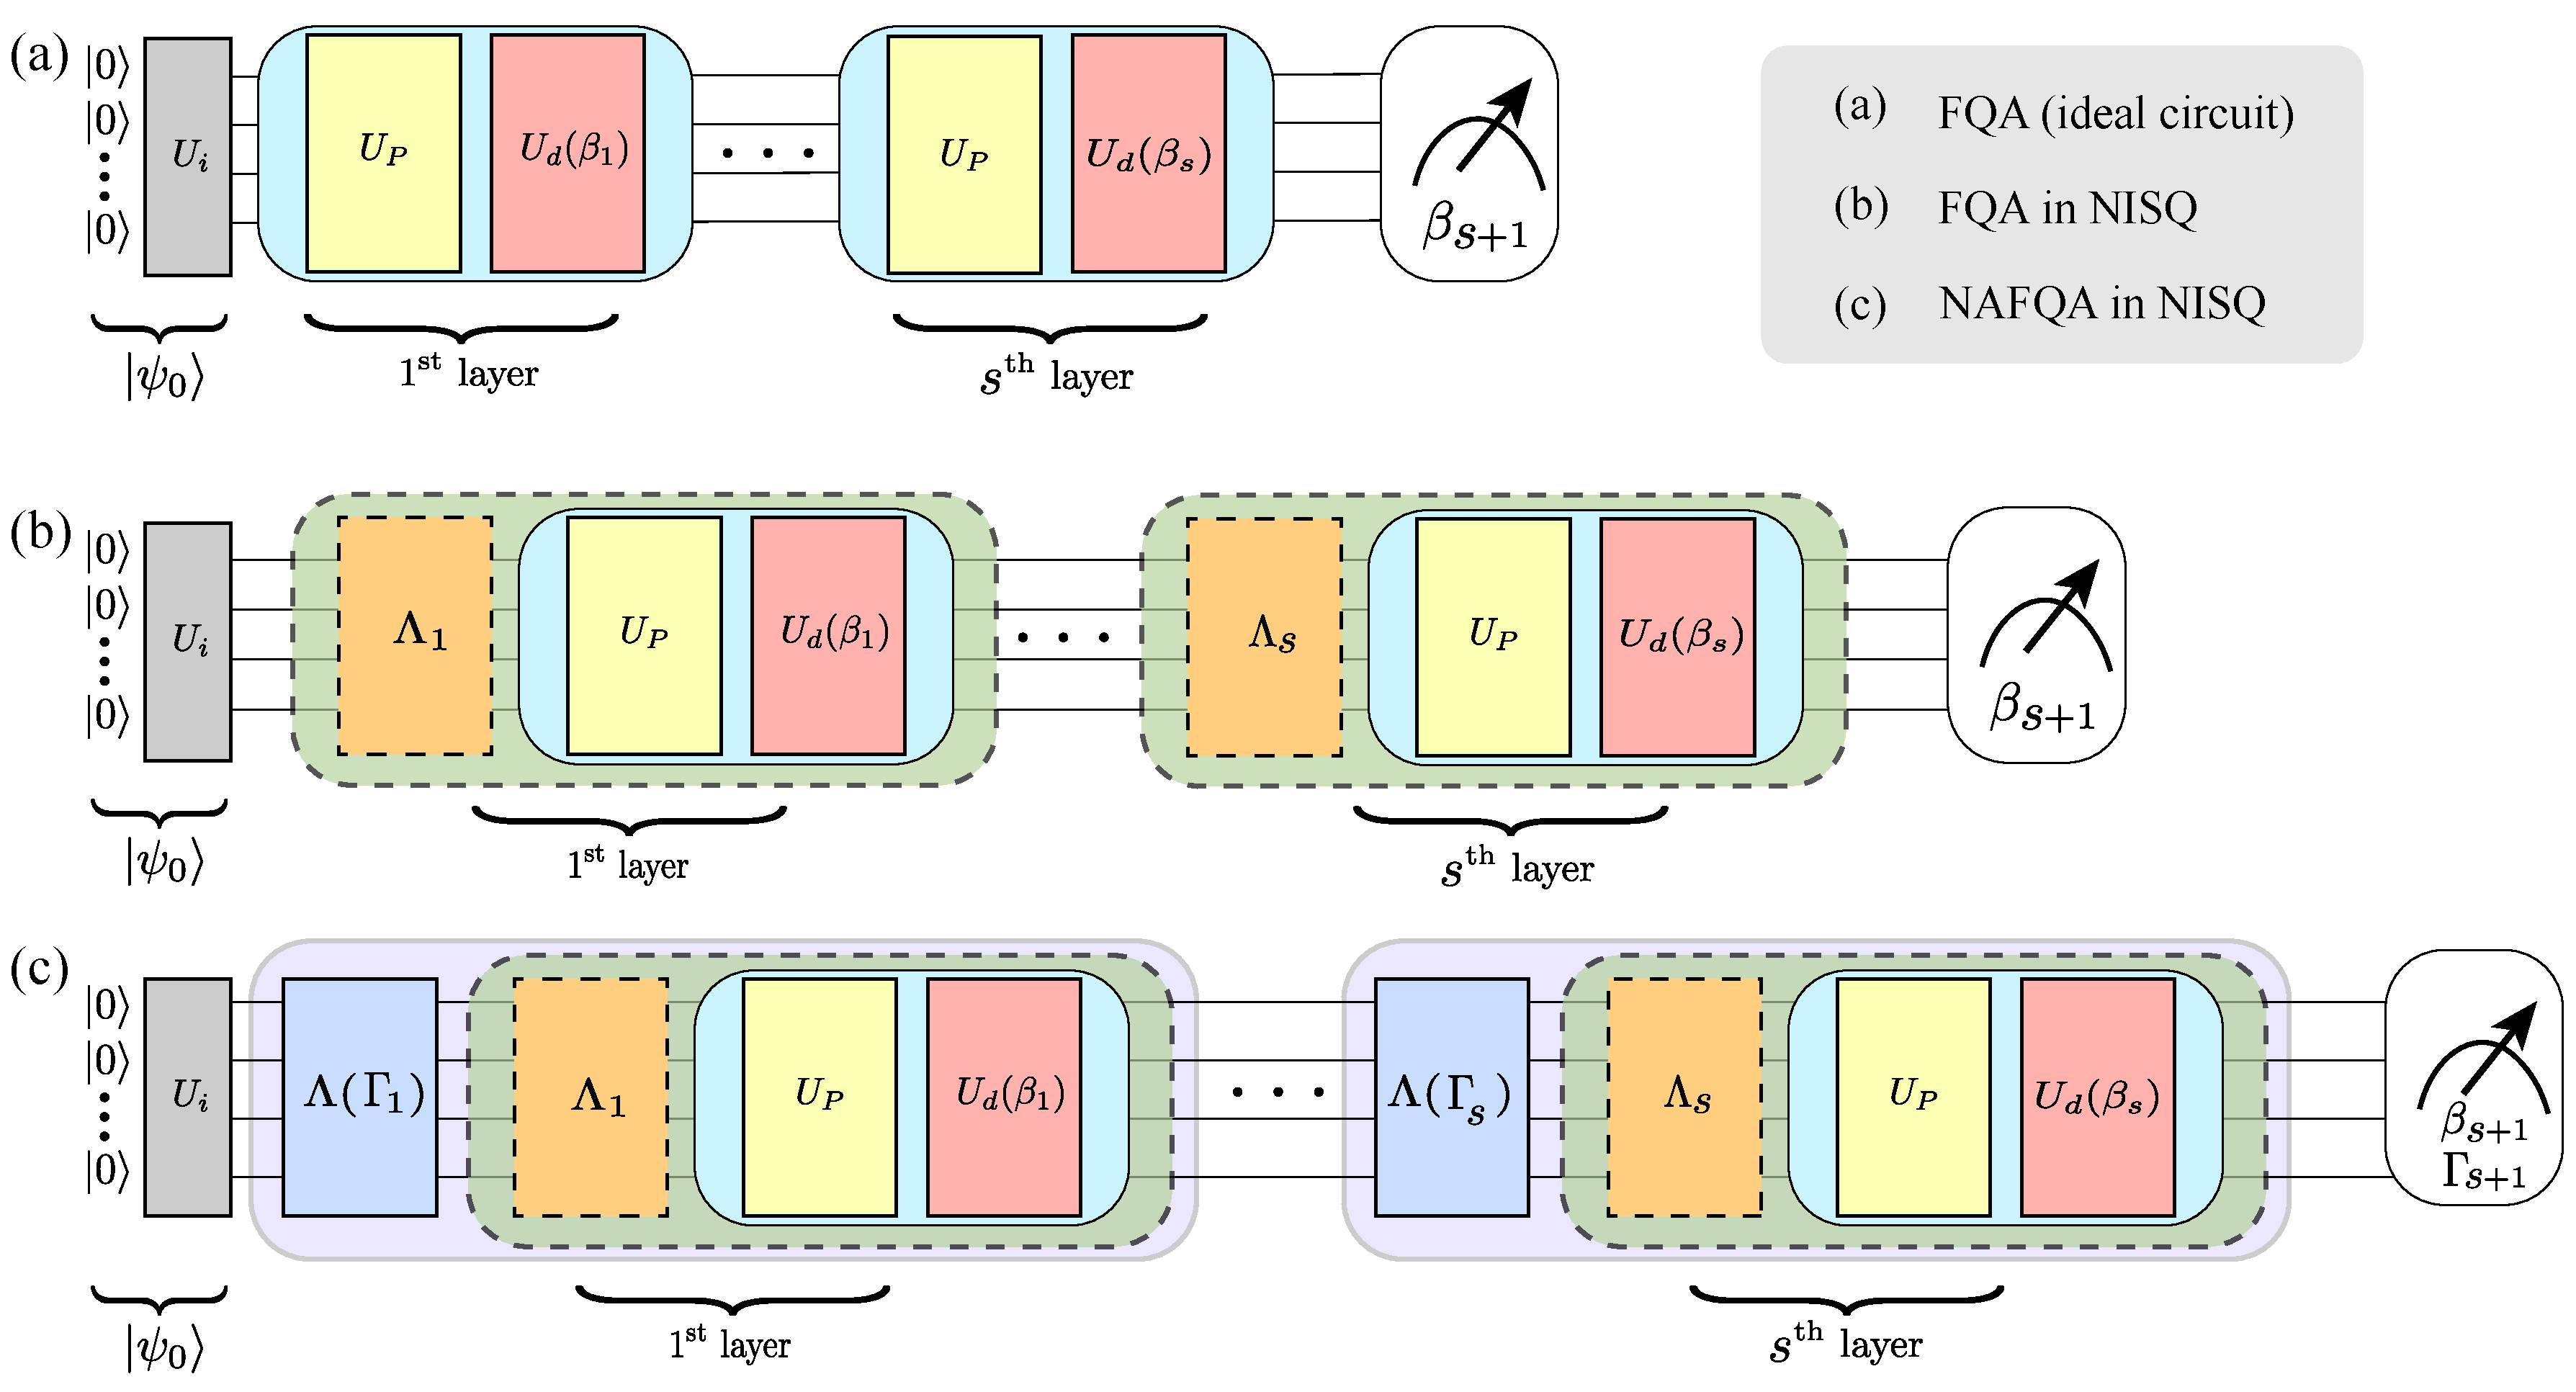
\includegraphics[scale=0.28]{final_plots/schematicv1.pdf} 
    \caption{\textbf{Schematic diagram of FQA in ideal, FQA in NISQ, and NAFQA in NISQ devices.}~(a) Ideal implementation of FQAs in a noiseless quantum computer consisting of $s$ Trotter layers. (b) Actual implementation of FQAs in NISQ devices where the ideal layer containing $U_p$ and $U_d(\beta_i)$ is interleaved with the inherent noise channel $\Lambda_s$. The dashed line represents the intrinsic device noise, over which the user generally has no control. (c) Our NAFQA algorithm is shown to use noise to drive an OQS simulation by introducing an additional noise map $\Lambda(\Gamma_s)$ derived from the feedback law. Note that the noise channels $\Lambda$ represent non-unitary evolutions and can be obtained via the stochastic unravelings of the GKSL master equation.} \label{Fig: Schematic_plot}
\end{figure*}

\subsection*{Quantum Lyapunov controlled feedback-based quantum algorithm}~Quantum Lyapunov control (QLC) is the founding principle behind recently developed FQAs designed for closed many-body systems. The QLC is a robust method that steers the dynamics of a quantum system towards a desired target state by tuning the Hamiltonian parameters. This is particularly applicable to finding approximate solutions to combinatorial problems or the ground state of many-body quantum Hamiltonians~\cite{SarovarPRL2022, Magann_PRA_2022, Dalcco_2024, RKMalla_PRR_2024, Larsen_prr, Shao_PhysRevA_2024}. For a closed quantum system described by a problem Hamiltonian $H_p$, the density matrix $\rho$ evolves according to the von Neumann equation $d \rho/dt = -i [H(t), \rho]$, where the time-dependent Hamiltonian $H(t) = H_p + \beta(t) H_d$, includes a control parameter $\beta(t)$ and a control Hamiltonian $H_d$. To ensure convergence towards the ground state, one should impose the Lyapunov condition $\frac{d}{dt} \braket{H_p} \leq 0,~ \forall t \geq 0$, which leads to
\begin{equation}
    \frac{d}{dt} \braket{H_p} = \beta(t) \braket{\psi(t) | i[H_d, H_p] | \psi(t)} = \beta(t) A(t) \leq 0,\label{closed_system}
\end{equation}
where $A(t) = \braket{\psi(t) | i[H_d, H_p] | \psi(t)}$. The above inequality can be satisfied by choosing an appropriate $\beta(t)$, and a convenient choice is $\beta(t) = - A(t)$. {This ensures a monotonic decrease in energy at all time steps. However, LaSalle's invariance principle~\cite{LaSalle1976} guarantees only convergence to the largest invariant subset of $\left\{\rho : \frac{d}{dt}\langle H_p\rangle = 
0\right\}$, which may include excited eigenstates of $H_p$. Under the sufficient conditions of Ref.~\cite{Magann_PRA_2022} (discussed later in the paper), asymptotic convergence to the ground state can be established. Nevertheless, ground-state convergence is observed numerically even when these conditions are not satisfied~\cite{SarovarPRL2022, Magann_PRA_2022, RKMalla_PRR_2024, 
Dalcco_2024, Larsen_prr}.}

FQA employs a Trotterized version of QLC, where the evolution time $t$ corresponds to discrete layers in a quantum circuit. A lower bound for $\beta(t)$ is derived in the Supplementary Information (SI) and is given by $\beta(t) \geq - \frac{\sqrt{||H_p||_{\Delta} } ~ \sqrt{||H_d||_{\Delta} }}{2}$, where $||\cdot||_{\Delta} $ is the semi-norm of an operator. Similarly, a bound for the Trotter step $dt$ can be obtained in terms of the spectral norms of $H_p$ and $H_d$ as, $dt \leq \frac{1}{4 ||H_p|| ||H_d||^2}$~\cite{Larsen_prr}. We note that statistical errors in estimating expectation values do not accumulate over time, despite uncertainties in determining $\beta(t)$ in each run. The overall uncertainty in statistical errors scales as $\frac{1}{\sqrt{M}}$, where $M$ is the number of repetitions for each measurement~\cite{RKMalla_PRR_2024}.

\begin{figure*}[t!]
    \begin{tabular}{c c}
    \centering
    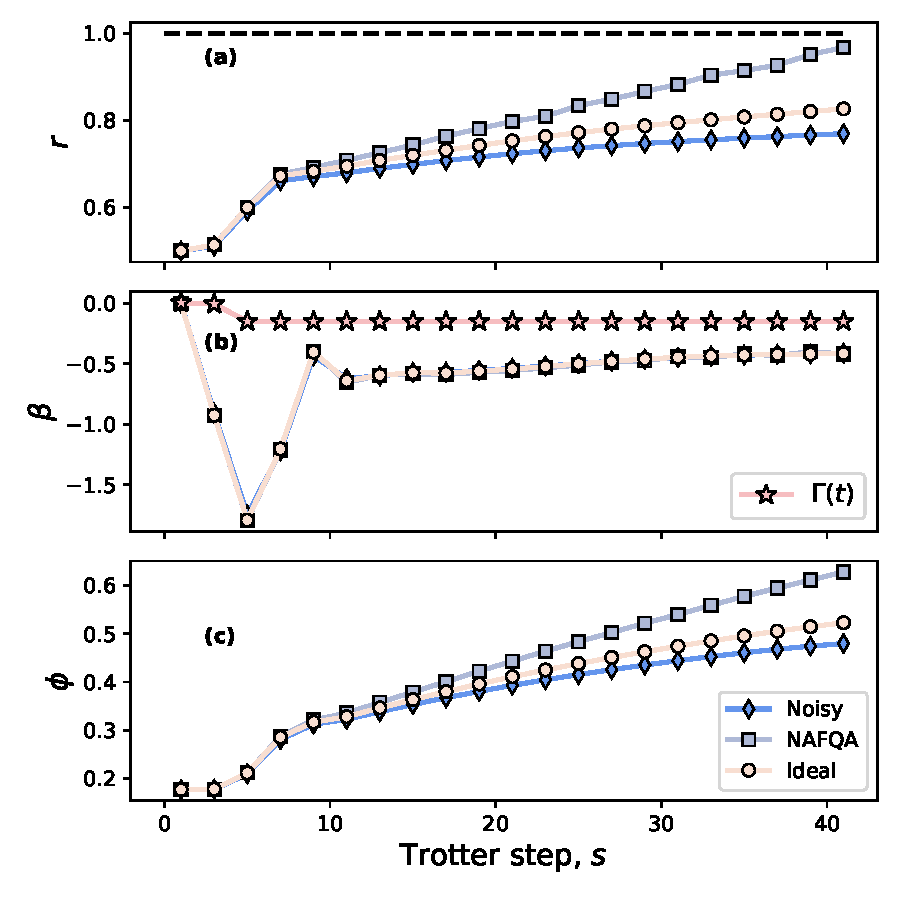
\includegraphics[scale=0.58]{final_plots/Maxcut_5q.pdf} & 
    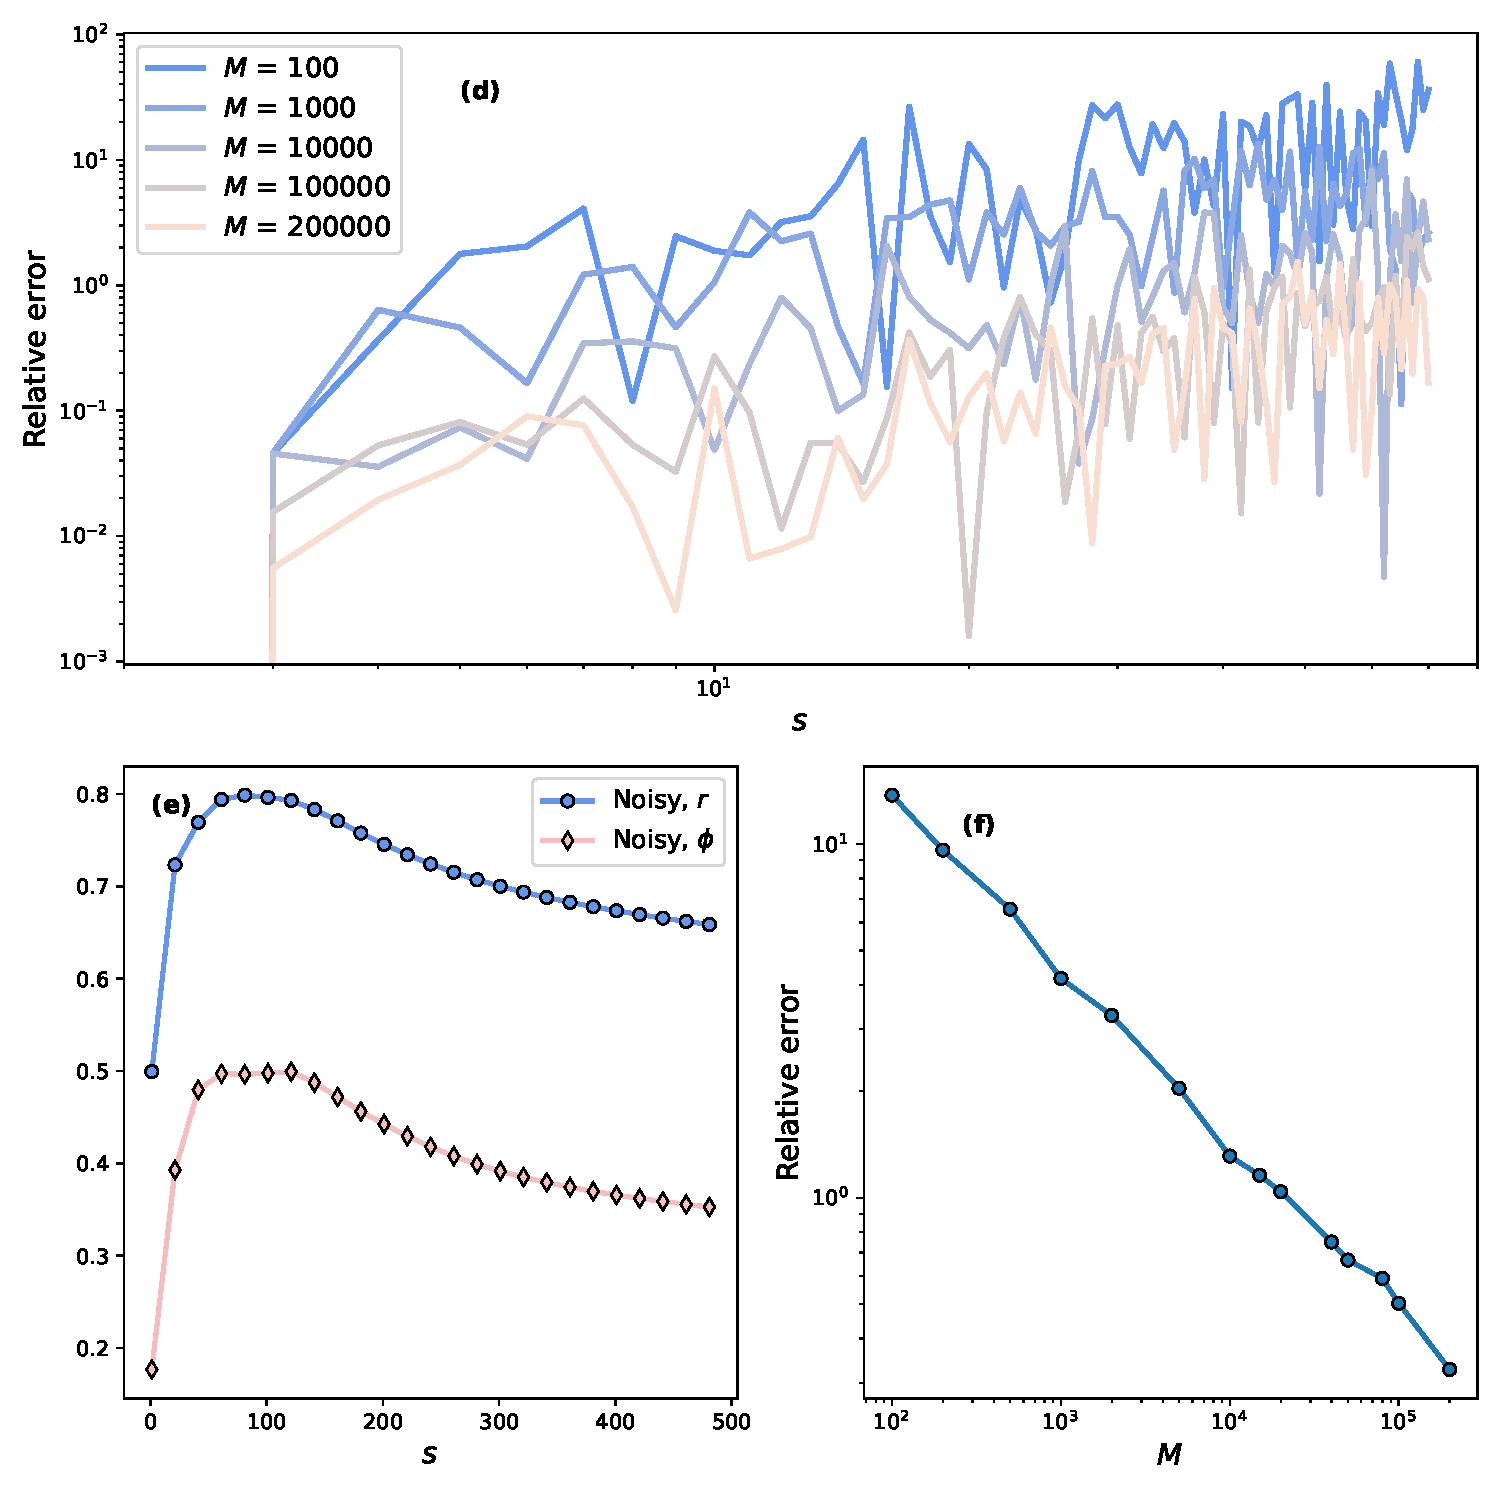
\includegraphics[scale=0.347]{final_plots/large_s.pdf}
    \end{tabular}
    \caption{\textbf{Numerical results for the 5-qubit Maxcut problem.}
    (a) The approximation ratio $r$, (b) the control terms $\beta(t)$ and $\Gamma(t)$, (c) the success probability $\phi$ as a function of the Trotter step with a fixed time step $dt = 0.07$. The inset in (b) shows $\Gamma(t)$ for the Pauli error term $IIYII$, whereas all the other Pauli terms' error probabilities are set to zero.  (d) Relative error as a function of the number of layers in the double logarithmic scale with several numbers of trajectories, $M$. (e) $r$ and $\phi$ at large times demonstrate the non-monotonic behavior. (f) Time averaged relative error as a function of $M$. }\label{one_decay_op}
\end{figure*}
% ntraj = 100000
% s = 41


\subsection*{Noise-assisted feedback-based approach}~The intrinsic noise of NISQ devices can be modeled using the Markovian theory of OQS~\cite{vandenBerg2023_natphys, Ferracin2024efficiently}, and can be written in the canonical form of the GKSL master equation~\cite{Breuer_book},
\begin{equation}
    \frac{d \rho}{dt} = -i [H, \rho] + \mathcal{D}_{\text{int}} [\rho]\label{rho_evolution}.
\end{equation}
The dissipator $\mathcal{D}_{\text{int}} [\rho]$ accounts for the system-environment coupling and is expressed as $\mathcal{D}_{\text{int}} [\rho] = \sum_i (L_i \rho L_i^\dagger - \frac{1}{2} L_i^\dagger L_i \rho - \frac{1}{2} \rho L_i^\dagger L_i )$, where the dissipation rates are absorbed into the Lindblad operators $L_i$.

To integrate the QLC into the OQS framework, we require that the rate of change of energy corresponding to the problem Hamiltonian $H_p$ must be negative,  
\begin{equation}
    \frac{d}{dt} \braket{H_p} = \beta(t)  \braket{i[H_d, H_p]} + \text{Tr}(\mathcal{D}_{\text{int}} [\rho] H_p) \leq 0. \label{open_system}
\end{equation}
The first term is similar to Eq.~\eqref{closed_system}, whereas the second term can be expanded as
\begin{equation}
\begin{split}
    \text{Tr}(\mathcal{D}_{\text{int}} [\rho] H_p) & = \sum_i \braket{ L_i^\dagger H_p L_i } - \sum_i \frac{1}{2} \braket{ \{H_p, L_i^\dagger L_i\} } & =\braket{\mathcal{D_{\text{int}}^{\dagger}}[H_p]},\label{superoperator_D}
\end{split}
\end{equation}
where $\{{A}, {B} \}$ denotes the anti-commutator of two operators ${A}$ and ${B}$. Thus, it reduces to the expectation value with respect to $\rho$ of the adjoint of the dissipator acting on $H_p$.  In the case of a pure dephasing channel, with the Lindblad operator $L \propto H_p$, Eq.~\eqref{superoperator_D} vanishes~\cite{wiseman2010quantum}, and we arrive at a Lyapunov condition that is similar to that introduced for closed quantum systems in Eq.~\eqref{closed_system}.

Randomized compiling or Pauli twirling have been proposed and experimentally realized to simplify the device noise as stochastic Pauli noise channels~\cite{Blatt_nat_comm_2019, vandenBerg2023_natphys, Kim2023}, as discussed in Eq.~\eqref{gen_pauli_channel}. Using this technique, the dissipator takes the form~\cite{EmersonPRA2016, Blatt_nat_comm_2019} 
\begin{equation}
    \mathcal{D}_{\text{int}} [\rho] = \sum_{k\in \mathcal{K}} \lambda_k (P_k \rho P_k^{\dagger} - \rho),\label{pauli_channel}
\end{equation}
where $L_k = \sqrt{\lambda_k} P_k$, and $\mathcal{K}$ is the selected set of local Pauli operators $\{P_k\}_{k\in\mathcal{K}}$ with associated error probabilities $\{\lambda_k\}_{k\in\mathcal{K}}$. The correlated noise in large quantum circuits can be modeled as a sparse channel and is given by~\cite{vandenBerg2023_natphys}
\begin{equation}
    \Lambda(\rho) = \text{exp}[\mathcal{D}_{\text{int}}](\rho) = 
    \prod_{k\in\mathcal{K}} \left( \omega_k \cdot + (1-\omega_k) P_k \cdot P_k^{\dagger} \right) \rho, \label{noise_channel_Lambda1}
\end{equation}
where $\omega_k = (1+e^{-2\lambda_k})/2$.  Here, $\mathcal{K}$ represents the local noise interactions of the quantum device, which is governed by the qubit-coupling topology. 
We assume on physical grounds a sparse model, in which the number of Pauli noise operators scales polynomially in the number of qubits $N$, i.e., $|\mathcal{K}| \ll 4^N-1$. 
In addition, although accurately characterizing noise remains an active area of research~\cite{PRXQuantum_Zoller_2022, Chen2023}, we further assume that the noise in NISQ devices can be reliably learned. Using Eq.~\eqref{pauli_channel},  Eq.~\eqref{open_system} becomes
\begin{equation}
\begin{split}
    \frac{d}{dt} \braket{H_p} & = \beta(t)  \braket{i[H_d, H_p]} 
    & + \sum_{k\in \mathcal{K}} \lambda_k \left(\braket{ P_k^\dagger H_p P_k } - \braket{H_p}\right) \leq 0. \label{lyapunov_lambda}
\end{split}
\end{equation}
{The second term in Eq.~\eqref{lyapunov_lambda} can be bounded as $\sum_{k\in \mathcal{K}} \lambda_k \left(\braket{ P_k^\dagger H_p P_k } - \braket{H_p}\right) \leq 2 ||H_p|| \sum_{k\in \mathcal{K}} \lambda_k \equiv \Lambda_\mathrm{noise} $ where $||\cdot||$ denotes the spectral norm; see SI. The second term can} be positive and is responsible for the deviation from the monotonic decrease in $\langle H_p \rangle$ and may explain the non-monotonic behavior of the energy as a function of the circuit depth in prior quantum hardware simulations~\cite{SarovarPRL2022, RKMalla_PRR_2024}.  


{
\begin{proposition}
(FQA with noise). Under the feedback law $\beta(t)= -A(t)$, the energy derivative satisfies $\frac{d}{dt}\langle H_p \rangle \leq -A(t)^2 + \Lambda_\mathrm{noise}$. The energy decreases monotonically if and only if $A(t)^2 \geq \Lambda_\mathrm{noise}$. Once $A(t)^2 < \Lambda_\mathrm{noise}$, the system enters a noise-dominated regime and the monotone descent guarantee is lost, precluding convergence to the ground state under the standard FQA feedback law alone.
\label{prop:fqa_noise}
\end{proposition}}

{Proposition~\ref{prop:fqa_noise} shows that the noise term $\Lambda_\mathrm{noise}$ sets a fundamental limit on the performance of FQA in NISQ devices.} One natural question arises: can making $\beta(t)$ more negative, accelerate convergence to the ground state? The answer is no. Intrinsic noise in quantum devices effectively heats the system, resulting in a mixed final state when FQAs are run on NISQ devices. Consequently, the true ground state cannot be reached in this manner. Similar questions can also be asked to increase the Trotter step $dt$ (instead of decreasing $\beta(t)$); however, the answers remain the same. In addition, the parameters cannot be arbitrarily large or small, and there is a bound for the $\beta(t)$ and $dt$ values that will depend on the choices of $H_p$, $H_d$~\cite{Magann_PRA_2022, Larsen_prr}; see SI. We demonstrate these statements numerically in Fig.~\ref{beta_change_purity} and discuss these aspects in more detail later in the paper. This observation motivates the development of an improved cooling strategy, which we outline below.

Alternatively, one may view this as suppressing deviations (the second term in Eq.~\eqref{lyapunov_lambda}) by dynamically adjusting the error probabilities over time, or, equivalently, across the layers of the quantum circuit. Here, we introduce an additional Lyapunov control that depends on the modified error probabilities $\{\Gamma_k(t)\}_{k\in\mathcal{K}}$, such that $\Gamma_k(t) = - C_k(t)$, where $C_k(t) = \left(\braket{ P_k^\dagger H_p P_k } - \braket{H_p}\right)_t$. For consistency, we keep the standard Lyapunov condition on $\beta(t)$, i.e., $\beta(t) = -A(t)$. 

{
\begin{theorem}
\label{thm:nafqa}
(NAFQA monotone descent). Under the joint feedback law $\beta(t) = 
-A(t)$ and $\Gamma_k(t) = -C_k(t)$ for all $k \in \mathcal{K}$, 
substituting into Eq.~\eqref{lyapunov_lambda} yields
\begin{equation}
    \frac{d}{dt}\langle H_p \rangle = -A(t)^2 - \sum_{k\in\mathcal{K}} 
    C_k(t)^2 \leq 0,\label{nafqa_descent}
\end{equation}
where both terms are non-positive. Consequently,
\begin{equation}
    \langle H_p \rangle_t \leq \langle H_p \rangle_0, \quad \forall\, 
    t \geq 0,
\end{equation}
with equality if and only if $A(t) = 0$ and $C_k(t) = 0$ for all $k \in \mathcal{K}$. This guarantee holds regardless of the Pauli noise coefficients 
$\{\lambda_k\}$, the system size $N$, or the circuit depth $s$, and constitutes a hardware-independent monotone descent unavailable to noisy FQA (Proposition~\ref{prop:fqa_noise}).
\end{theorem}

\begin{proof}
Substituting $\beta(t) = -A(t)$ and $\Gamma_k(t) = -C_k(t)$ into Eq.~\eqref{lyapunov_lambda}, the energy derivative becomes $\frac{d}{dt}\langle H_p \rangle = -A(t)^2 - \sum_{k\in\mathcal{K}} C_k(t)^2$,
which is non-positive at all $t \geq 0$.
\end{proof}

Under NAFQA, the total layer-dependent rate becomes $\Gamma_k(t) = \lambda_k + \nu_k(t)$, where $\nu_k(t)$ is the engineered rate, which will be introduced later in the paper. Therefore, Eq.~\eqref{lyapunov_lambda} generalizes to
\begin{equation}
    \frac{d}{dt}\langle H_p\rangle = \beta(t)\langle 
    i[H_d,H_p]\rangle + \sum_{k\in\mathcal{K}} 
    \Gamma_k(t)\bigl(\langle P_k^\dagger H_p 
    P_k\rangle - \langle H_p\rangle\bigr).\label{eq:nafqa_update}
\end{equation}
Substituting the joint feedback law $\beta(t) = -A(t)$ and $\Gamma_k(t) = -C_k(t)$ into this expression yields Eq.~\eqref{nafqa_descent}.

By LaSalle's invariance principle~\cite{LaSalle1976}, the NAFQA trajectory converges to the largest invariant subset of
\begin{equation}
    \mathcal{S} = \left\{\rho\,:\, A(t) = 0 \;\text{and}\; C_k(t) = 0 
    \;\forall\, k\in\mathcal{K}\right\}.
\end{equation}
The invariant set $\mathcal{S}$ is restricted by two conditions, each acting on a different part of the NAFQA dynamics:
\begin{itemize}
    \item[\textbf{(C1)}] The 
    expectation value $\braket{i[H_d,H_p]} = 0$ only at energy eigenstates of $H_p$. This holds when $\{H_p, H_d\}$ generate $\mathfrak{su}(2^N)$~\cite{JURDJEVIC1972, Altafini2002}, leaving no non-trivial invariant subspace under the unitary dynamics. This is similar to the conditions~(1)--(3) of Ref.~\cite{Magann_PRA_2022} for closed-system FQA. \label{C1}
    
    \item[\textbf{(C2)}] For every excited eigenstate $|E_n\rangle$ 
    ($n > 0$), $\exists\, k \in \mathcal{K}$ such that 
    $\braket{E_n|P_k^\dagger H_p P_k|E_n} \neq E_n$, so that the 
    dissipative term excludes excited eigenstates from 
    $\mathcal{S}$~\cite{Wang2010}. This is generically satisfied when 
    $\{P_k\}$ do not simultaneously diagonalize $H_p$.
\end{itemize}
}
{Both conditions are checkable a priori from the operator structure alone, without knowledge of the eigenvalues or eigenstates of $H_p$. Condition~(C1) is checked by computing the rank of the Lie algebra generated by $\{iH_p,iH_d\}$ via repeated commutators. Condition~(C2) reduces to verifying $[P_k,H_p]\neq 0$ for at least one $k\in\mathcal{K}$, which holds generically whenever the noise model contains Pauli operators outside the stabilizer group of $H_p$. Whether these conditions extend to guarantee the ground state convergence for mixed states under the full open-system dynamics is an open question and can be explored in future works.}

The time-local master equation corresponding to Eq.~\eqref{eq:nafqa_update} can be expressed as 
\begin{equation}
    \frac{d \rho(t)}{dt} = -i [H(t), \rho(t)] + \sum_{k\in \mathcal{K}} \Gamma_k(t) (P_k \rho(t) P_k^{\dagger} - \rho(t)),\label{na--qlc}
\end{equation}
where the sign of $\Gamma_k(t)$ determines whether the noise map is Markovian or non-Markovian. The bounds for the decay rates $\Gamma_k(t)$ are derived in the SI in terms of purity and fidelity between the initial and final states. However, one can obtain Eq.~\eqref{na--qlc} in a quantum device following Eq.~\eqref{non_Markovian-ckt}. The corresponding master equation reads
\begin{equation}
    \frac{d \rho(t)}{dt} = -i [H(t), \rho(t)] + \mathcal{D}_{\text{int}} [\rho(t)] + \mathcal{D}_{\text{eng}} [\rho(t)],\label{NAFQA-qlc}
\end{equation}
where the engineered dissipator takes the form $\mathcal{D}_{\text{eng}} [\rho(t)] = \sum_{k\in \mathcal{K}} \nu_k(t) (P_k \rho(t) P_k^{\dagger} - \rho)$, with time-dependent rates $\nu_k(t)$ that leads to $\Gamma_k(t) = \lambda_k + \nu_k(t)$. The overhead cost for this case, as derived in Ref.~\cite{Enod_PhysRevA_2021}, is given by
{\begin{equation}
    \mathcal{N} (T) = \text{exp}\left[\sum_{k\in \mathcal{K}} \int_0^T\left( |\nu_k(t)| - \nu_k(t) \right) dt\right].\label{error_mitigation_cost}
\end{equation}

We emphasize that $\mathcal{N}(T)$ is governed solely by the magnitudes $|\nu_k(t)|$ of the engineered negative rates, and is independent of the intrinsic device error probabilities $\{\lambda_k\}$. In our case, $\nu_k(t) \leq 0$ by the Lyapunov feedback law, the integrand satisfies $|\nu_k(t)| - \nu_k(t) = 2|\nu_k(t)|$, so the overhead reduces to $\mathcal{N}(T) = \exp\!\left[2\sum_{k\in\mathcal{K}}\int_0^T|\nu_k(t)|\,dt\right]$. In the limit $\nu_k \to 0$, $\mathcal{N}(T) \to 1$, and no additional sampling cost is incurred beyond the base FQA overhead~\cite{SarovarPRL2022}.} According to Hoeffding's inequality, the number of samples $M$ that ensures an average expectation value with error $\delta$ and probability $1-\epsilon$ is given by $M \propto \mathcal{N}^2\frac{\log(1/\epsilon)}{\delta^2}$~\cite{Jinzhao_Sun_PhysRevApplied_2021}. As a result, the sampling overhead scales as $\mathcal{N}^2$, incurring an increased cost due to the negativity of the rates to guarantee fixed precision. We note that the overhead scaling remains exponential in the number of Pauli noise operators $|\mathcal{K}|$ within the sparse model assumption. In this sense, our scheme does not circumvent the need for advancing quantum error correction. 

\subsection*{Quantum circuit implementation of NAFQA}
The quantum circuit for NAFQA is built iteratively: the parameters for the $s+1$-th layer are determined from measurement on a quantum circuit built up to the $s$-th layer. Each layer contains the unitaries $U_p$, $U_d(\beta_s)$, and the noise channel $\mathcal{F}_s = \Lambda_s \circ \Lambda'_s$, as shown in Fig.~\ref{Fig: Schematic_plot} (c). For the next layer, we define the control field $\beta_{s+1} = - A_{s}$ and the modified noisy map $\mathcal{F}_{s+1} (\cdot) = \Lambda \circ \Lambda' (\{\Gamma(s+1)\})$ that contains error probabilities $\Gamma(s+1)_k = - \{(C(s)_k\}_{k\in \mathcal{K}}$, where the mathematical form of the noise channel $\Lambda'(\cdot)$ is given in Methods. The parameters $C(s)$ and $\Gamma(s+1)$ are used for the Trotter steps $s$ and $s+1$, respectively. The method to simulate the decay rates $\Gamma$ in an ideal quantum circuit at the Trotter step $s$ is summarized in Algorithm \ref{algor_pseudo}, and is further discussed in Methods. We repeat the process for a finite number of Trotter steps $s$ and find that this feedback-based procedure ensures a monotonic decrease in energy with additional Lyapunov controls, where the noise channels drive the system faster toward the virtual ground state.

% \begin{figure}[t!]
%     \centering
%     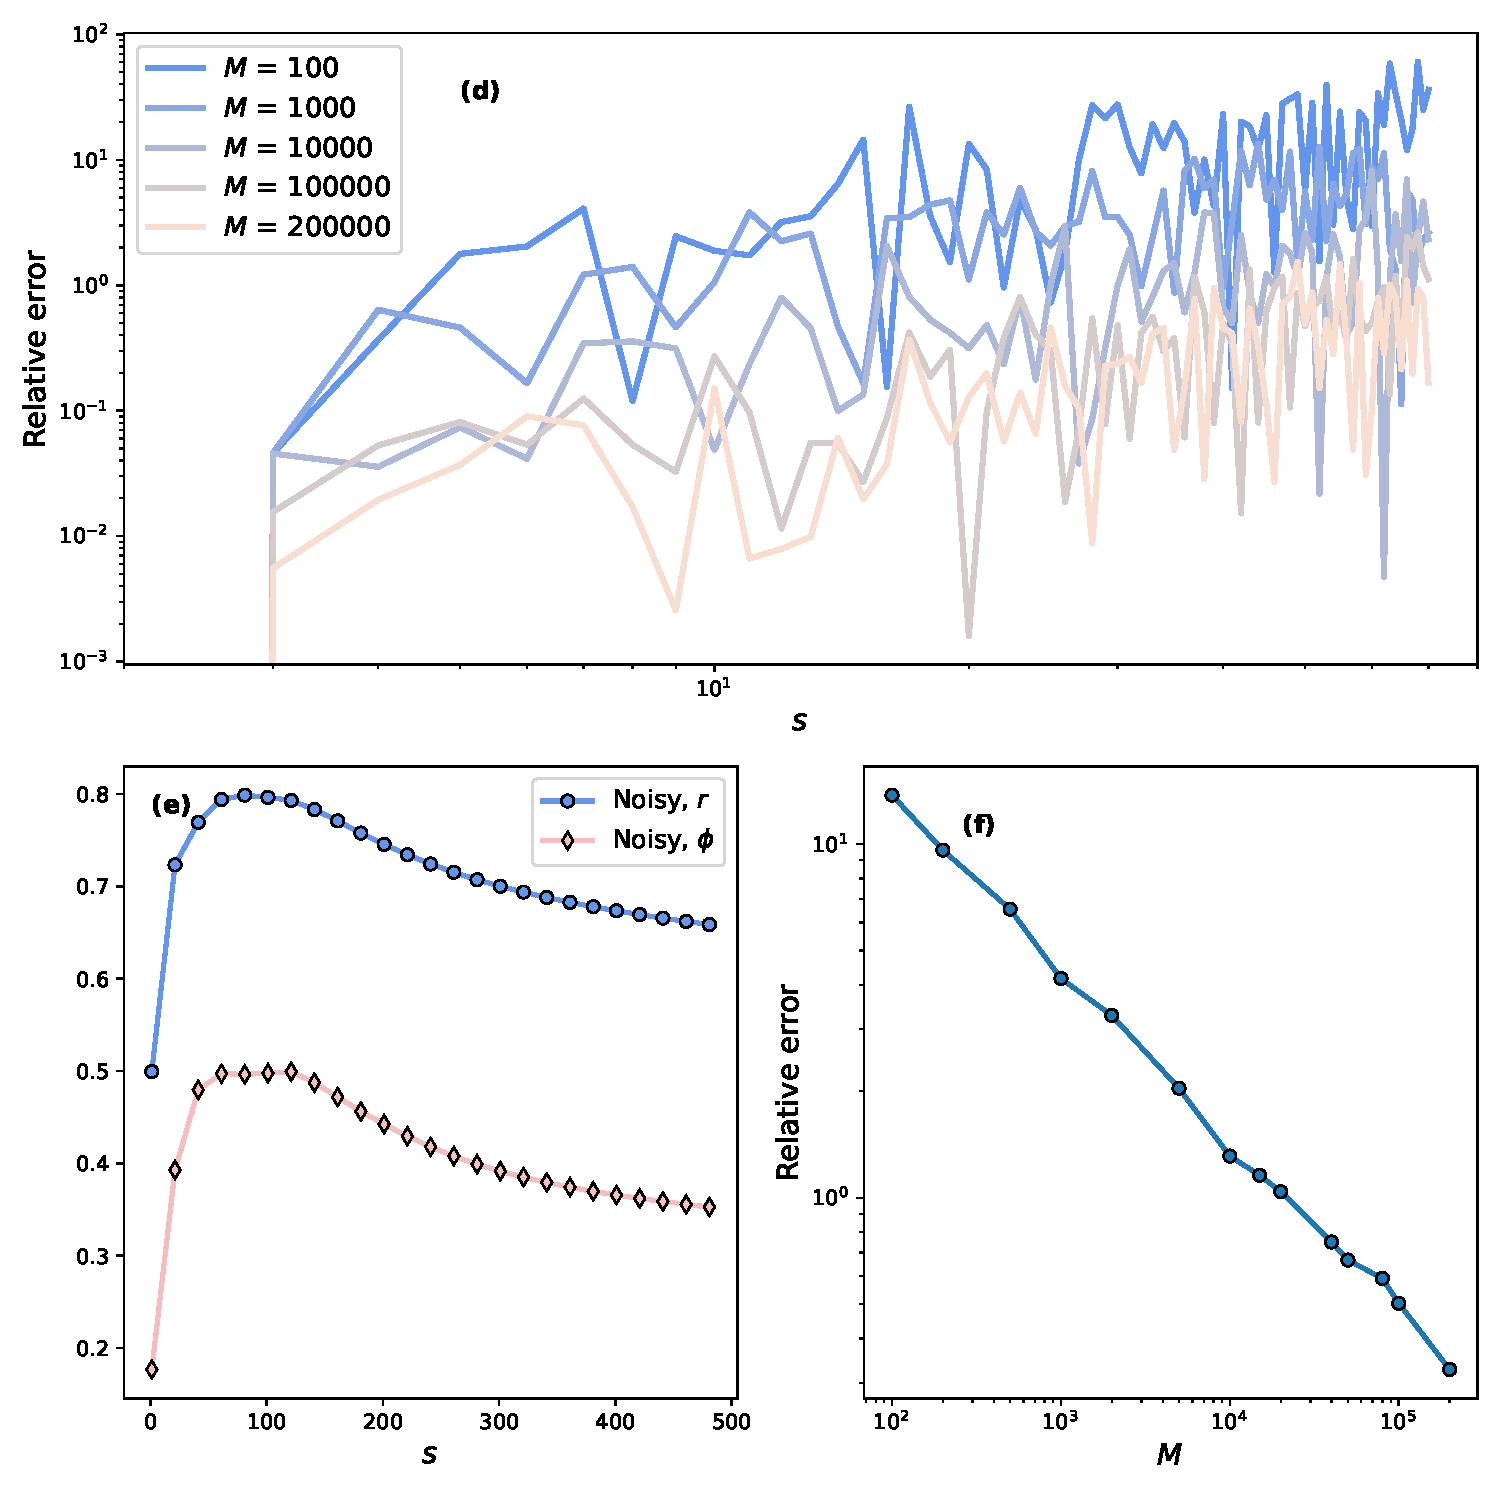
\includegraphics[scale=0.31]{final_plots/large_s.pdf} 
%     \caption{\textbf{Numerical results for the 5-qubit Maxcut problem.}
%     }\label{large_s}
% \end{figure}

% To kick-start the feedback process, we initialize the first layer of the quantum circuit by incorporating the inherent noise in the quantum circuit. Using randomized benchmarking~\cite{EmersonPRA2016, Blatt_nat_comm_2019}, we modeled the noise as stochastic Pauli noise channels and characterized its error probabilities with the cycle error reconstruction method~\cite{Flammia2020}. Here, we have assumed that the sparse noise model given in Eq.~\eqref{noise_channel_Lambda1} is the same for each layer, which leads to $\Lambda = \Lambda_1 = \Lambda_2 = \cdots = \Lambda_s$. This assumption is justified since the unitaries corresponding to $H_p$ are fixed and the unitary corresponding to $H_d$ contains only single-qubit terms. However, to accurately implement noise, one must learn the noise models $\Lambda_s$ at each layer.

To kick-start the feedback process, we initialize the first layer of the quantum circuit by incorporating the inherent noise as stochastic Pauli-noise channels. Here, we have assumed that the Pauli sparse noise model given in Eq.~\eqref{noise_channel_Lambda1} is the same for each layer, which leads to $\Lambda = \Lambda_1 = \Lambda_2 = \cdots = \Lambda_s$. This assumption is justified since the unitary corresponding to $H_p$ is fixed and the unitary corresponding to $H_d$ contains only single-qubit terms. However, to accurately implement the intrinsic noise, one must learn the noise models $\Lambda_s$ at each layer.

A key feature of our NAFQA protocol is that the coefficients $\Gamma_k(t)$ can take negative values. While such values correspond to unphysical noisy channels, they nonetheless satisfy the Lyapunov condition in the OQS framework. This type of OQS dynamics with negative $\Gamma$ can be implemented, as described in Algorithm \ref{algor_pseudo}.

\begin{figure*}[t!]
    \begin{tabular}{c c c}
    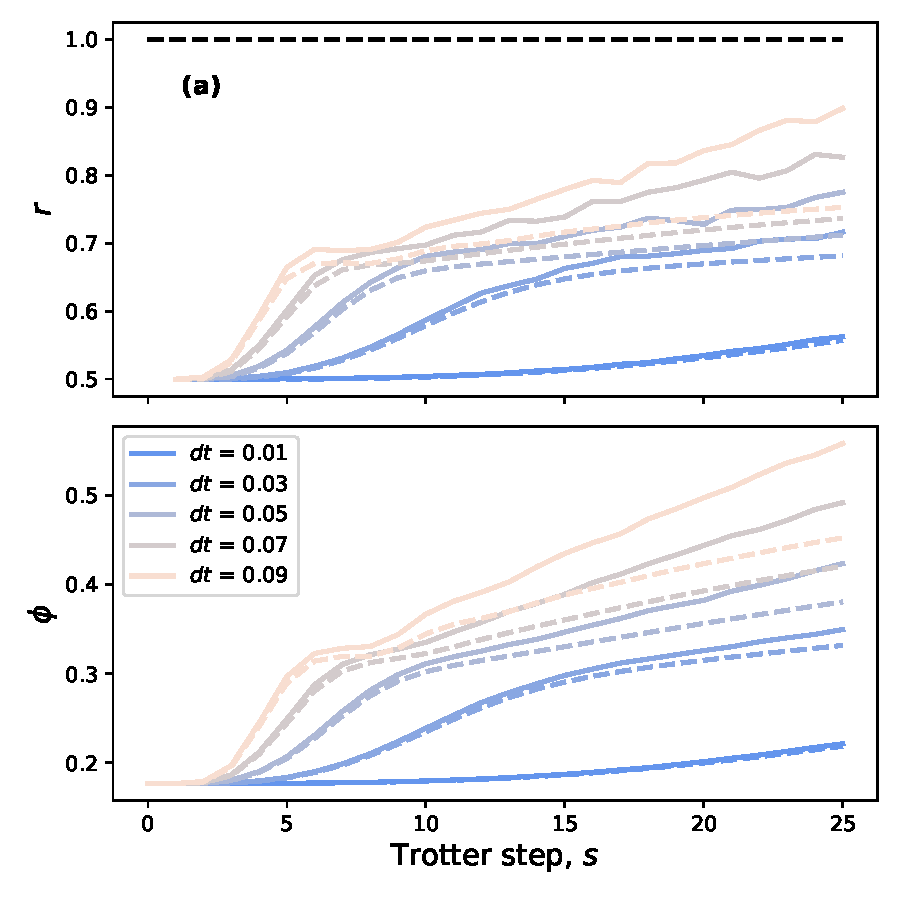
\includegraphics[scale=0.38]{final_plots/demo_2.pdf} &
    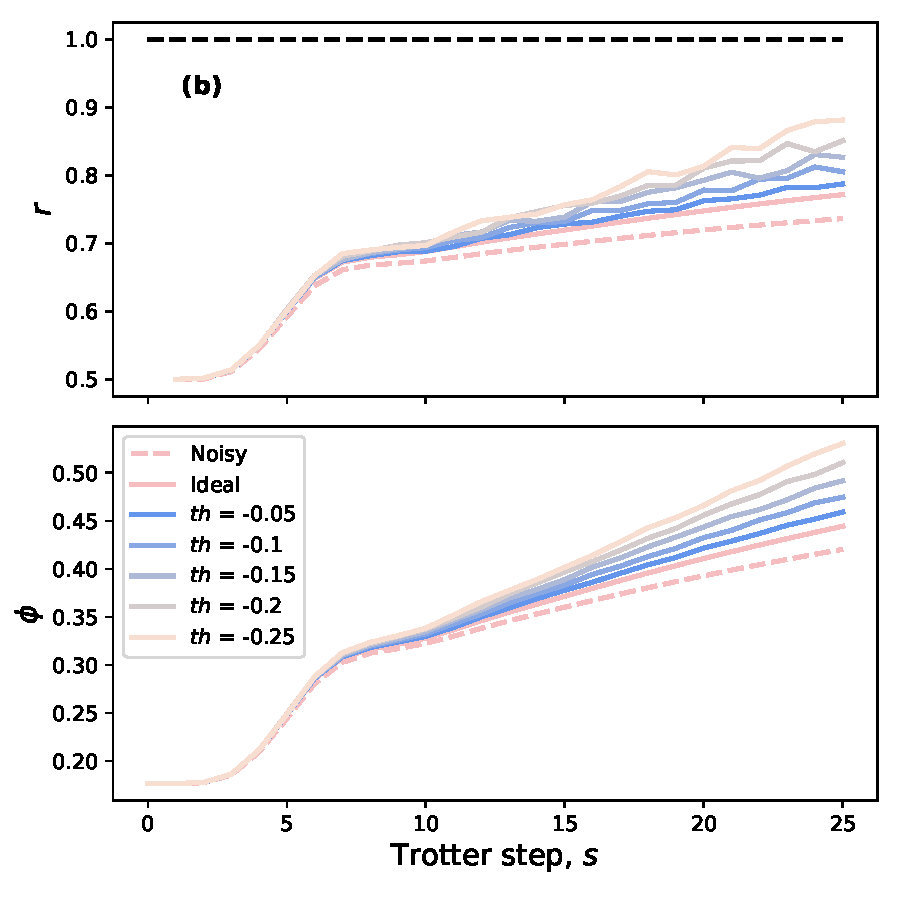
\includegraphics[scale=0.38]{final_plots/demo_3.pdf} &
    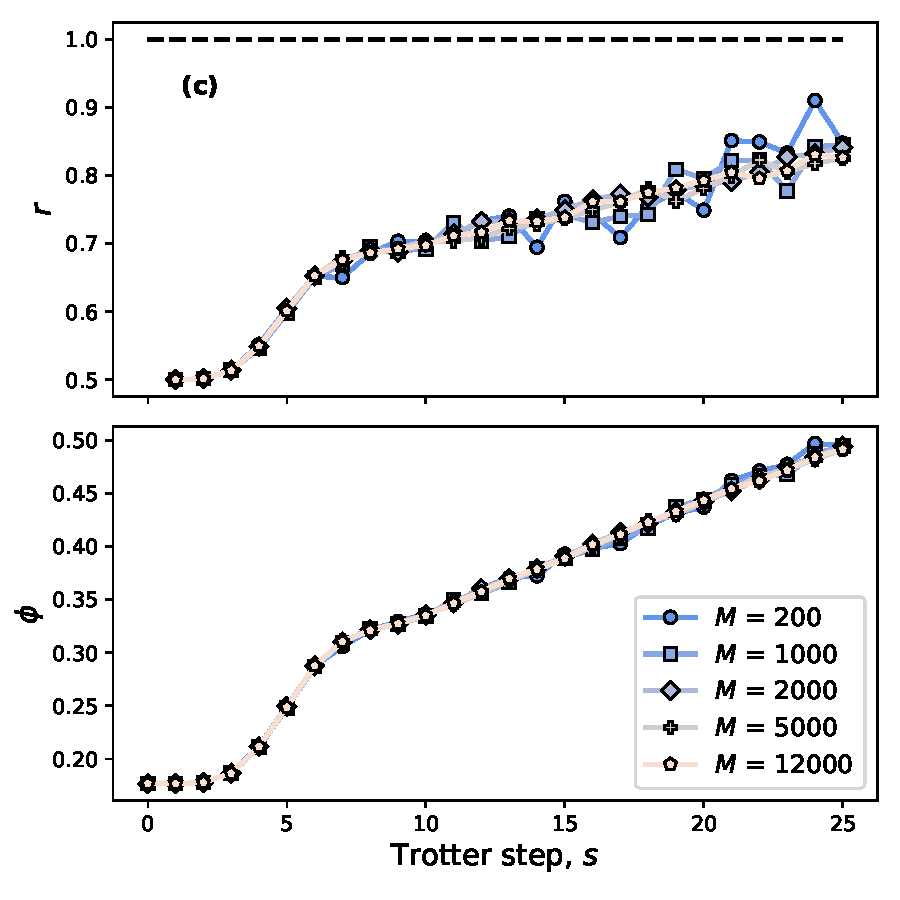
\includegraphics[scale=0.38] {final_plots/ntraj_demo.pdf}
    \end{tabular}
    \caption{\textbf{Time evolution of approximate ratio $r$ and success probability $\phi$ with  different parameters involved in the NAFQA protocol.} We considered several cases: (a) varying the time steps $dt$ with a fixed sample size, $M = 12000$, (b) different threshold values of $\Gamma(t)$ from $\text{th} = -0.05$ to $\text{th} = -0.25$ with $dt = 0.07$ and $M = 12000$. The dotted and solid lines indicate the noisy and NAFQA evolutions, respectively. (c) Various numbers of samples $M$ are used for a fixed time step $dt = 0.07$ and threshold value of $\text{th} = -0.15$ .}\label{Fig: panel plot}
\end{figure*}

\begin{algorithm}[H]
\caption{Quantum circuit simulation for non-Markovian dynamics}
\KwIn{Initial state $|\psi_m^{(s-1)}\rangle$, noiseless ideal unitary $U_s$ at the $s^{\text{th}}$ Trotter layer, number of samples $M$, Trotter-step $dt$}
% \KwOut{Final state $\rho_f$}

\For{$1\leq m \leq M$}{
        {1. Compute  $\ket{\psi_m}^{(s)} = U^{(s)} \ket{\psi_m}^{(s-1)}$ \\


        2. Sample $P_k$ with probability $r_k dt$, with $r_k = {|\Gamma_k|}$  \\
        Compute  $\ket{\psi_m}^{(s)} = \sqrt{|\Gamma_k|}P_k \ket{\psi_m}^{(s)}/ {\sqrt{r_k}}$ \\
        Update sign: $s^{(s)}_m \gets s^{(s-1)}_m \cdot \frac{\Gamma_k}{|\Gamma_k|}$\\
        
        \textbf{Or}\\

        2. Sample $I$ with probability $r_{\text{res}} = 1-\sum_k r_k dt $ \\
        Compute  $\ket{\psi_m}^{(s)} = \ket{\psi_m}^{(s)} / {\sqrt{r_{\text{res}}}}$\\
        Update sign: $s^{(s)}_m \gets s^{(s-1)}_m (+1)$}\\

    3. Compute: $\rho^{(s)}_m = s^{(s)}_m \cdot |\psi_m^{(s)}\rangle \langle \psi_m^{(s)}|$ , 
}
$\mathcal{N}^{(s)} = \sum_{m=1}^{{M}} s_m^{(s)} \braket{\psi_m^{(s)} | \psi_m^{(s)}}$.\\
\Return $\rho^{(s)}_f = \frac{1}{\mathcal{N}^{(s)}} \sum_{m=1}^{M} \rho^{(s)}_m$. \label{algor_pseudo}
\end{algorithm}

\begin{figure}[t!]
    \centering 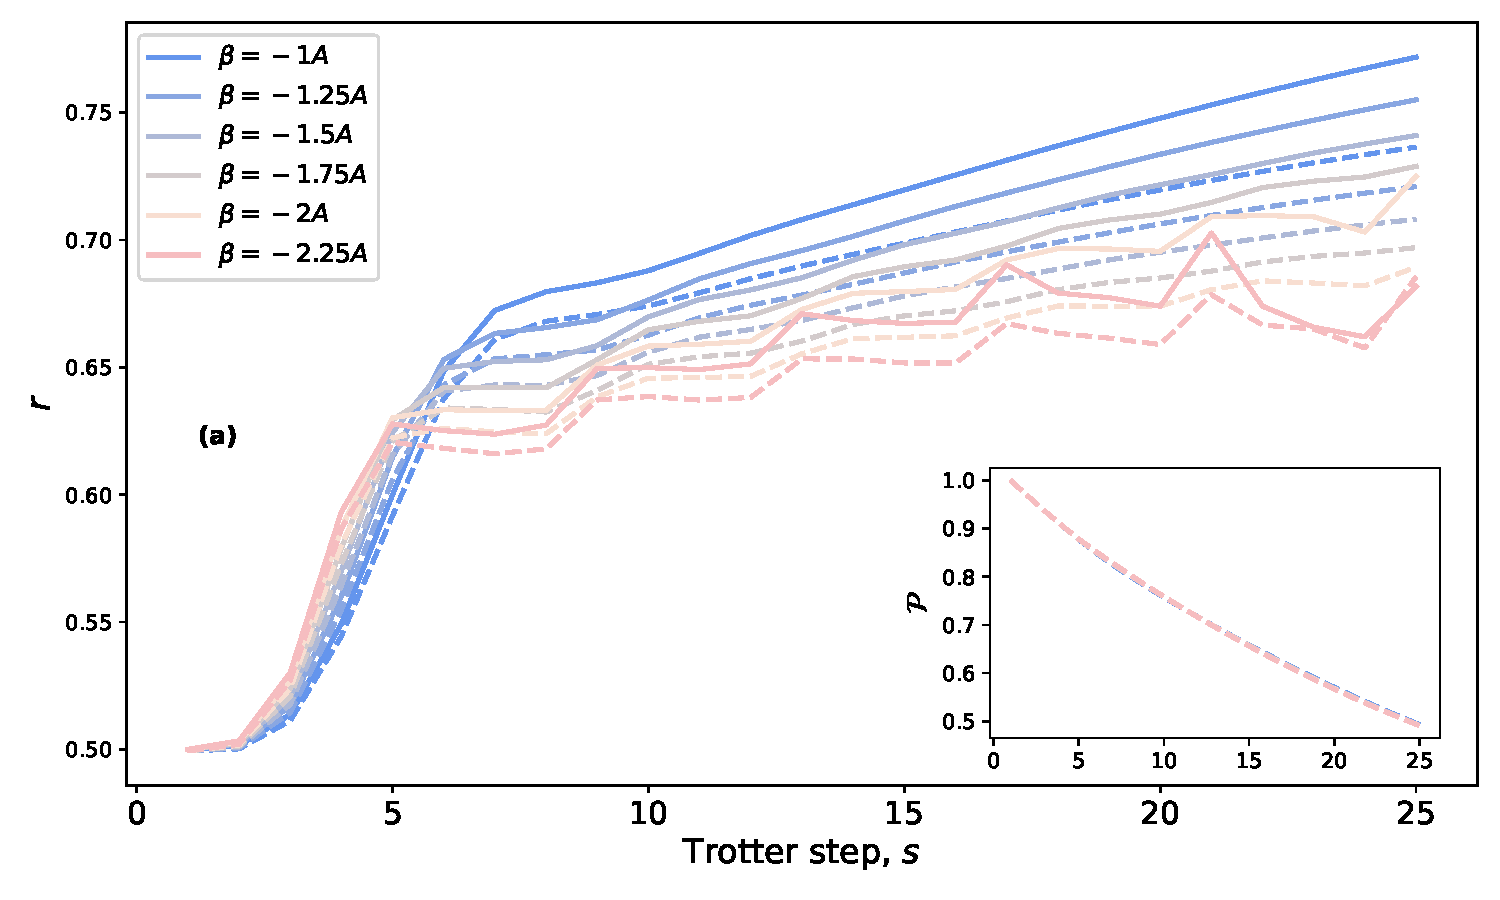
\includegraphics[scale=0.33]{final_plots/change_beta.pdf} 
    \centering 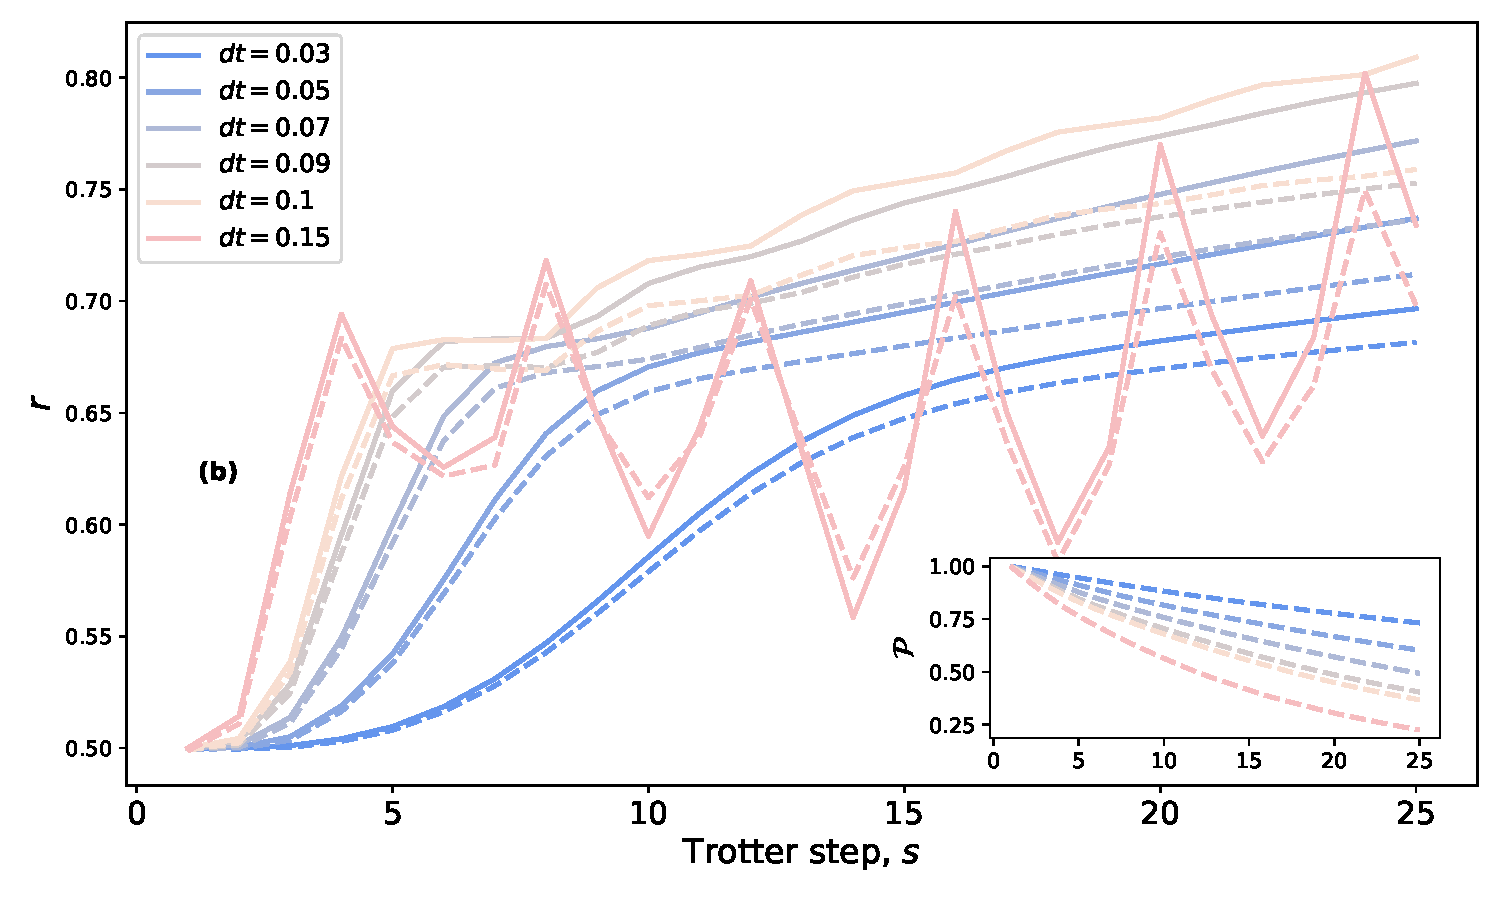
\includegraphics[scale=0.33]{final_plots/change_dt.pdf} 
    \caption{\textbf{Performance of FQA in the closed and open quantum system framework.} Approximation ratio $r$ for the 5-qubit Maxcut problem with varying the (a) control field $\beta$ and (b) Trotter-step $dt$. Panel (a) is shown for the fixed Trotter step $dt = 0.07$, whereas panel (b) is illustrated for $\beta = - A$. The dotted and solid lines represent the noisy and ideal evolutions, respectively. The inset shows the purity $\mathcal{P}$ of the noisy evolutions as a function of Trotter steps.}\label{beta_change_purity}
\end{figure}


We now proceed to discuss the protocol for calculating the expectation values with negative decay rates in experiments. The idea behind QPD is to represent an ideal circuit as a quasiprobabilistic mixture of noisy circuits~\cite{Gambetta2017PRL}. With this, one can efficiently measure the bias-free expectation value with correct classical post-processing of the measurement outcomes. This idea can be extended to decompose any arbitrary physical or nonphysical map $\Lambda'_s(\rho)$. It can be expressed as a linear combination of noisy operations $\{\mathcal{\tilde{U}}\}$ that can be implemented on quantum hardware, 
\begin{equation}
    \Lambda'_s(\rho) = \sum_i \eta_{s,i} \mathcal{\tilde{U}}_i(\rho) \approx \mathcal{N} _s \sum_i \frac{|\eta_{s,i}|}{\mathcal{N} _s} \text{sgn} ~ (\eta_{s,i}) \mathcal{\tilde{U}}_i,\label{samp_over}
\end{equation}
where $\eta_{s,i}$ can be negative, $\text{sgn}(\cdot)$ denotes the sign function, and $\mathcal{N} _s = \sum_i |\eta_{s,i}|$ is the sampling overhead that satisfies $\mathcal{N}_s \geq 1$. The probability $p_{s, i} = \frac{|\eta_{s,i}|}{\mathcal{N}_s}$ is non-negative and sums up to 1. Given an input state $\rho$, the expectation value of an operator $O$ after the desired channel $\Lambda'_s(\rho)$ can be written as
\begin{equation}
    \braket{O}_{\text{eff}} = \text{tr}[O\Lambda'_s(\rho)] = \mathcal{N}_s \sum_i p_{s,i} ~ \text{sgn} (\eta_{s,i}) \text{tr}[O~\mathcal{\tilde{U}}_i(\rho)]. \label{qpd_eqn}
\end{equation}

The QPD is implemented as follows. For each channel $\Lambda'_s(\rho)$, the noisy operation $\mathcal{\tilde{U}}_i$ is sampled with probability $p_{s,i}$, and the measured expectation value is multiplied by the parity, $\text{sgn}(\eta_{s,i})$. After sampling over multiple estimators, the computed unbiased expectation value $\braket{O}_{\text{eff}}$ is obtained after multiplying with the overhead coefficient $\mathcal{N}_s$, as given in Eq.~\eqref{qpd_eqn}. Note that the measurement $\text{tr}[O~\mathcal{\tilde{U}}_i(\rho)]$ taken after each sample is executed on a quantum computer and the final expectation value of the observable $\braket{O}_{\text{eff}}$ is calculated on a classical computer after scaling with the signs and the sampling overhead. However, the computation of the expectation value comes with an additional overhead as the variance of the estimator increases by a factor of $\mathcal{O}(\mathcal{N} ^2)$~\cite{Jinzhao_Sun_PhysRevApplied_2021}. The total overhead for $L$-layers becomes $\mathcal{N}_{\text{tot}} = \prod_{s = 1}^{L}\mathcal{N} _s$. QPD has a runtime that scales roughly as $(1 + \frac{15}{8} \epsilon)^{NL}$, where $N$ is the number of qubits, $L$ is the circuit depth, and $\epsilon$ is the two-qubit depolarizing error~\cite{vandenBerg2023_natphys}. This exponential scaling does not mean that these protocols are without value; in fact, lowering hardware error rates $\epsilon$ can provide a promising pathway to quantum advantage~\cite{aharonov2025importanceerrormitigationquantum, zimborás2025mythsquantumcomputationfault}. Rapid developments in reducing variance and run-time cost using tensor network error mitigation~\cite{fischer2024dynamicalsimulationsmanybodyquantum} and
shaded light cones~\cite{eddins2024lightconeshadingclassicallyaccelerated} are also demonstrated, opening new doors for the introduction of algorithms incorporating these techniques.

Although we model noise using a general stochastic Pauli channel, we emphasize that our approach is broadly applicable and can be implemented with any noise model. The only requirement is that the noise that affects each layer must be known or characterized in advance. A more detailed discussion of noise models beyond stochastic Pauli channels, particularly those involving amplitude and phase damping, is presented later in the paper.

\subsection*{Optimization problem}~We demonstrate the effectiveness of our NAFQA algorithm by applying it to two illustrative examples, the Maxcut problem and the spin glass Hamiltonians. The initial state $\ket{\psi_0}$ is prepared in the state $\ket{+}^{\otimes N}$ for a $N$ qubit system. The performance of our algorithm is measured based on two figures of merit: the approximation ratio, $r = {\braket{H_p}}/{\braket{H_p}_{\text{min}}}$ and the success probability, $\phi = \bra{\psi_{\text{gs}}} \rho \ket{\psi_{\text{gs}}}$, where $\rho$ is the density matrix and $\ket{\psi_{\text{gs}}}$ is the ground state obtained by diagonalizing the problem Hamiltonian $H_p$. Both figures of merit $r$ and $\phi$ vary from 0 to 1, with $r = \phi \approx 1$ corresponding to the approximate solution of the ground state.

As a first example, we consider the unweighted Maxcut problem, where the Hamiltonian for $N$ qubits is given by $H_p = -\sum_{i,j\in \mathcal{E}} \frac{1}{2}(1 - Z_iZ_j)$. The control Hamiltonian is chosen as $H_d = \sum_{j = 1}^{N} X_j$. Given $H_p$ and $H_d$, the commutator in Eq.~\eqref{closed_system} takes the form $i[H_d,H_p] = \sum_{i,j\in \mathcal{E}} Y_iZ_j + Z_i Y_j$. Here, $X_j$, $Y_j$, and $Z_j$ are the Pauli operators that act on the qubit $j$. {We note that the Max-Cut graph topology and the device noise model are independent choices. The graph is a 5-qubit linear chain with edge set $E = \{(1,2),(2,3),(3,4),(4,5)\}$, motivated by the original FQA work of Ref.~\cite{SarovarPRL2022}, whereas the stochastic Pauli noise probabilities $\{\lambda_k\}$ are taken from the IBM-Vigo emulator, as shown in Fig.~\ref{Fig: twilring_plot}.}

In Fig.~\ref{one_decay_op}, we present the results of the NAFQA algorithm and compare them with simulations of the FQA designed for closed-system dynamics, both in the presence and absence of noise. ``Ideal" refers to noiseless FQA simulations (Fig.~\ref{Fig: Schematic_plot} (a)), while ``Noisy" simulations correspond to the FQA simulations with the stochastic Pauli noise channels (Fig.~\ref{Fig: Schematic_plot} (b)). Noisy simulations are equivalent to solving Eq.~\eqref{rho_evolution} with the learned error probabilities $\{\lambda\}$ of quantum hardware, while still enforcing the Lyapunov condition defined for an isolated system, as introduced in Eq.~\eqref{closed_system}. We learned the error probabilities $\{\lambda\}$ of the 5-qubit IBM-Vigo simulator using Qiskit~\cite{Qiskit2021} and plotted them in Fig.~\ref{Fig: twilring_plot} (c). The schematic circuit diagrams for FQA and NAFQA on NISQ devices are shown in Figs.~\ref{Fig: Schematic_plot} (b) and (c), respectively. 

We begin by characterizing the approximation ratio, $r$, and the success probability, $\phi$, as a function of $s$. We observed that with NAFQA, $r$ ($\phi$) increases from $0.5 ~ (0.17)$ at $s = 0$ to $0.97$ ($0.64$) at $s = 41$. In contrast, for the noisy (ideal) simulations, we obtain $r \approx 0.77 (0.82) $ and $\phi \approx 0.48 (0.53)$ at $s = 41$ (Fig.~\ref{one_decay_op} (a) and (c)). This corresponds to an improvement of $26\%$ for $r$ and an improvement of $33\%$ for $\phi$ with our methods compared to the noisy FQA simulations. For the NAFQA simulations, we modify only one Pauli term as a function of $s$ and set the error probabilities of all other terms to zero. This shows that even a single modified error probability can accelerate the system's evolution towards the virtual ground state, highlighting the effectiveness and adaptability of our algorithm. Figure~\ref{one_decay_op} (b) shows the time dependence of the control parameters $\beta$ and $\Gamma$. Enforcing QLC in NAFQA yields negative $\Gamma$ rates, which are obtained by the non-Markovian Monte Carlo solver in Qutip~\cite{JOHANSSON_qutip_2013}. 

The noisy simulations demonstrate non-monotonic behavior in both $r$ and $\phi$ (Fig.~\ref{one_decay_op} (e)), and it decays to $r ~ (\phi) \approx 0.65 (0.35)$ after $s = 500$ steps. This is expected as they do not satisfy the QLC condition; see Eq.~\eqref{lyapunov_lambda}. {The statistical precision of NAFQA} with respect to the number of samples $M$ grows exponentially with time, as shown in Eq.~\eqref{error_mitigation_cost}. To quantify this behavior, we define the relative error $\delta$ as the deviation from the normalized trace of $1$ as, $\delta = (\text{Tr} -1 ) \times 100$, where $\text{Tr}$ is the trace of the state. Figure~\ref{one_decay_op} (d) shows that $\delta$ increases with $s$ for a fixed number of samples, and decreases in a particular $s$ as $M$ increases. Next, we plot the time-averaged $\delta$ as a function of $M$ on a double logarithmic scale, and it scales approximately as $\delta \propto 1/\sqrt{M}$. This verifies that running NAFQA at long timescales requires an exponentially large number of samples (Eq.~\eqref{error_mitigation_cost}). Therefore, it is not possible to show a convergence of $r$ and $\phi$ as a function of $s$.

The {statistical precision of NAFQA} depends on the magnitude of the negative decay rates as well (Eq.~\eqref{error_mitigation_cost}). To regulate the decay rates $\Gamma_k$, we establish a threshold of $-0.15$ as demonstrated in Fig.~\ref{one_decay_op} (b) i.e., if $\left(\braket{ P_k^\dagger H_p P_k } - \braket{H_p}\right) > 0.15$, we set $\Gamma_k = - 0.15$; otherwise, we assign $\Gamma_k (t)= - \left(\braket{ P_k^\dagger H_p P_k } - \braket{H_p}\right)_t$. We note that the choice of $-0.15$ as the threshold is arbitrary. However, a finite threshold value mitigates the need for a prohibitively large number of trajectories, which would otherwise increase the computational cost as $\Gamma_k$ decreases. 

We now proceed to examine the performance of NAFQA and compare it with noisy evolutions through a series of numerical simulations. Figure~\ref{Fig: panel plot} illustrates the behavior of $r$ and $\phi$ for different values of time steps $dt$, threshold value `$\text{th}$', and sample sizes $M$. Increasing the Trotter step $dt$ improves $\phi$ and $r$ monotonically as a function of $s$, as shown in Fig.~\ref{Fig: panel plot} (a). Decreasing the threshold value similarly increases the performance of the protocol, as seen in Fig.~\ref{Fig: panel plot} (b). Finally, Fig.~\ref{Fig: panel plot} (c) reveals that both $r$ and $\phi$ stabilize with increasing $M$, indicating that statistical errors do not accumulate and the protocol remains robust in the large-sample limit. 

We also demonstrate the performance of FQA in the ideal and noisy framework by varying the control field $\beta(t)$ and the Trotter-step $dt$, as illustrated in Fig.~\ref{beta_change_purity}. We find that making $\beta(t)$ more negative or increasing $dt$ speeds up evolution ($r$ and $\phi$ increase) for short times. However, there is a bound for both $\beta$ and $dt$, and one should not cross these limits. Otherwise, the parameters start to oscillate very frequently, and the FQA protocol does not work. Although we provide bounds on the parameters (see SI), tighter bounds would be desirable to optimize the choice of $\beta$ and $dt$, which could be investigated in future work. We note that simply making $\beta(t)$ more negative or increasing $dt$ does not solve the heating problem. 
Our results indicate that FQAs implemented on NISQ devices will inevitably evolve into mixed states and will not converge to their pure ground states.
This is verified by the monotonic decrease of the purity $\mathcal{P}(t) = \text{Tr}[\rho(t)^2]$, as shown in the insets in Fig. \ref{beta_change_purity}. Thus, our NAFQA protocol provides a practical approach to the computation of ground-state properties on NISQ devices.

\subsection*{Spin glass Hamiltonians}
We now present the performance of our algorithm for spin-glass Hamiltonians over several instances. {We consider an all-to-all spin-glass Hamiltonian for $N = 5$ qubits, expressed as $H_p = \sum_{m<n}J_{mn}Z_m Z_n + \sum_l h_l Z_l$, where the control Hamiltonian $H_d$ takes the form $H_d = - \sum_{j = 1}^{5} X_j$. With these choices of $H_p$ and $H_d$, the commutator becomes $i[H_d,H_p] =  -2 \left(\sum_{i<j}J_{ij} (Y_i Z_j + Z_i Y_j) + \sum_{i} h_i Y_i \right)$. The resulting mean and standard error of $r$, $\phi$, and $\beta$ are shown in Fig.~\ref{TFIM_plot}. The numerical simulations are performed over 25 instances (seeds 0 through 24) for 5000 trajectories. The coupling constants $J_{mn}$ and the transverse field strengths $h_l$ are randomly and independently drawn from a uniform distribution on $[-1,+1]$. As with the Maxcut problem, NAFQA exhibits monotone descent toward the ground-state properties for spin-glass instances. Noisy simulations are performed with the error probabilities given in Fig.~\ref{Fig: twilring_plot} (c), scaled by a multiplicative factor of 100. This amplification serves to emulate the effect of stronger noise or, equivalently, in the noise-dominated regime established by Proposition~\ref{prop:fqa_noise}, the accumulation of noise at circuit depths approximately 100 times larger than those simulated. The amplified noisy FQA results are presented solely to illustrate the qualitative long-time behavior predicted by Proposition~\ref{prop:fqa_noise}, namely irreversible drift toward a mixed state (which is very far away from the true ground state) once $A(t)^2 < \Lambda_\mathrm{noise}$. However, here we consider five additional Lyapunov controls that determine the modified error probabilities $\Gamma_k$ ($k = 1,2,3,4,5$), compared to only one for the Maxcut problem. As shown in Fig.~\ref{TFIM_plot}, a threshold of $-0.15$ is taken for all decay rates. We note that $\beta(t)$ varies smoothly throughout the simulations, and that the modified rates $\Gamma_k(t)$ are the key factors enabling the extraction of ground-state properties on shorter timescales. Additional numerical results for $N = 8$ qubits are provided in the SI, further corroborating the performance and robustness of NAFQA across system sizes. The data and code to reproduce all figures are publicly available at the GitHub repository~\cite{nafqa_kasturi}.}

\section*{Discussion}
NAFQA is conceptually distinct from dissipative ground-state preparation protocols~\cite{Verstraete2009, kraus_pra_2008, science_dissipation, lin_lin_review_2025, barbara_cooling} and from variational or feedback-based approaches augmented with error mitigation. Bath-engineering and dissipative cooling methods are designed for settings in which the Lindblad operators and decay rates are fixed, with the target state engineered as the unique steady state of the resulting Lindbladian. Such protocols are powerful but presuppose hardware capabilities such as controllable reservoir coupling, additional ancilla qubits, or analog tunability--that are not generally available on current NISQ devices. NAFQA addresses a complementary regime: it operates directly on native device noise, characterized via randomized compiling~\cite{EmersonPRA2016, Flammia2020, EmersonPRX2021}, and exploits it as a feedback-controlled computational resource without requiring any bath engineering or ancilla overhead. The feedback law is constructed entirely from the problem and driver Hamiltonians $H_p$, $H_d$, and the available Pauli noise operators $\{P_k\}$, making it adaptive to the noise present in the specific device. Furthermore, NAFQA is broadly compatible with existing noise characterization pipelines: the only prerequisite is a Pauli-twirled sparse noise model, which is already routinely produced by cycle benchmarking workflows~\cite{vandenBerg2023_natphys}.

The distinction from variational quantum algorithms (VQE) or FQA combined with probabilistic error cancellation (PEC) is equally fundamental: whereas PEC yields unbiased estimates of noiseless expectation values by suppressing device noise at exponential sampling cost~\cite{Gambetta2017PRL, Cai_QEM_2023}, QPD in NAFQA is used constructively to engineer non-Markovian dissipation with negative decay rates. Rather than canceling noise, NAFQA incorporates it into the Lyapunov feedback law, constituting a qualitatively different use of the quasiprobability framework. These complementary roles suggest that future hybrid protocols combining bath-engineering with feedback-adaptive noise control may be a fruitful direction, and recent advances in dissipative many-body ground-state preparation~\cite{lin_lin_review_2025, barbara_cooling} offer a tantalizing prospect for such combinations.

The net practical advantage of NAFQA over noisy FQA is not a reduction in sampling cost but the restoration of the monotone descent guarantee. Proposition 1 establishes that noisy FQA loses the monotone descent guarantee once $A(t)^2 < \Lambda_\mathrm{noise}$, precluding convergence to the ground state under the standard FQA feedback law alone. Theorem~1 establishes that NAFQA recovers unconditional, hardware-independent monotone descent at all circuit depths $s$ and system sizes $N$, independently of the device error probabilities $\{\lambda_k\}$, $N$, and $s$. The total sampling cost of NAFQA relative to the original FQA cost $\mathcal{N}_s^{\text{FQA}} = \mathcal{O}(mds)$ of Refs.~\cite{SarovarPRL2022, Magann_PRA_2022} is
\begin{equation}
    \mathcal{N}_s^{\text{NAFQA}} = \mathcal{O}\!\left(
    mds \cdot |\mathcal{K}| \cdot \mathcal{N}^2(s)
    \right),
    \label{eq:nafqa_cost}
\end{equation}
where $m$ is the number of samples per Pauli expectation value, $d$ is the number of Pauli terms in the commutator $i[H_d, H_p]$, and $|\mathcal{K}| \ll 4^N - 1$ under the sparse Pauli-Lindblad model. The factor $|\mathcal{K}|$ enters linearly while $\mathcal{N}^2$ is exponential in $|\nu_k|s$, regulated by the threshold $\nu_{\max}$. This exponential cost is the price paid for algorithmic correctness, in the same spirit as the overhead of the standard PEC for unbiased estimation of expectation values~\cite{vandenBerg2023_natphys}. The practical regime of utility is characterized by two conditions: $|\mathcal{K}|$ scales polynomially in $N$ (satisfied when noise operators follow the qubit connectivity~\cite{vandenBerg2023_natphys}), and $\nu_\mathrm{max}$ is chosen sufficiently small to keep $\mathcal{N}^2(s)$ tractable at the circuit depths of interest.

{Several limitations of NAFQA should be acknowledged explicitly. First, the protocol requires noise characterization as a necessary prerequisite: the Pauli-Lindblad error probabilities $\{\lambda_k\}$ must be learned via randomized compiling before the feedback law can be constructed. Second, the QPD implementation of the engineered negative rates incurs an exponential sampling overhead $\mathcal{N}^2(s)$ that grows with circuit depth, as established by Eq.~\eqref{error_mitigation_cost} and Eq.~\eqref{eq:nafqa_cost}. This overhead is fundamental in nature, structurally analogous to the fermionic sign problem in quantum Monte Carlo~\cite{Troyer_prl_2005} and is not a limitation of our particular implementation. The threshold $\nu_{\max}$ regulates this cost in practice, but accessing the statistically precise regime at large $s$ requires a sampling budget that grows exponentially, placing an inherent limit on the accessible circuit depths and making it more suitable for near-term quantum computers. Third, NAFQA is applicable when the sparse Pauli-Lindblad model holds, i.e., when the number of relevant noise operators $|\mathcal{K}|$ scales polynomially in $N$. While this may seem restrictive, recent experiments demonstrate that a sparse noise model with one- and two-local Pauli terms following the qubit topology captures the correlated noise in superconducting quantum processors and scales to large quantum devices~\cite{vandenBerg2023_natphys}. In this sense, NAFQA does not constitute an alternative to quantum error correction for large-scale, fault-tolerant computation.}

{This work opens several further avenues for future exploration. The control protocol for OQS could be extended to steer the system toward a decoherence-free subspace~\cite{Wang2010}; see SI. Our approach can also be explored beyond stochastic noise channels, particularly in the presence of both unital and non-unital noise or when noise is integrated directly with quantum gates~\cite{Bassi_prr_2023}. Applications may further extend to fast charging and discharging of quantum batteries~\cite{Shastri2025} and to rapid thermalization via shortcuts to adiabaticity~\cite{Alipour2020shortcutsto, Yin2022}.}

\begin{figure}[t!]
    \centering
    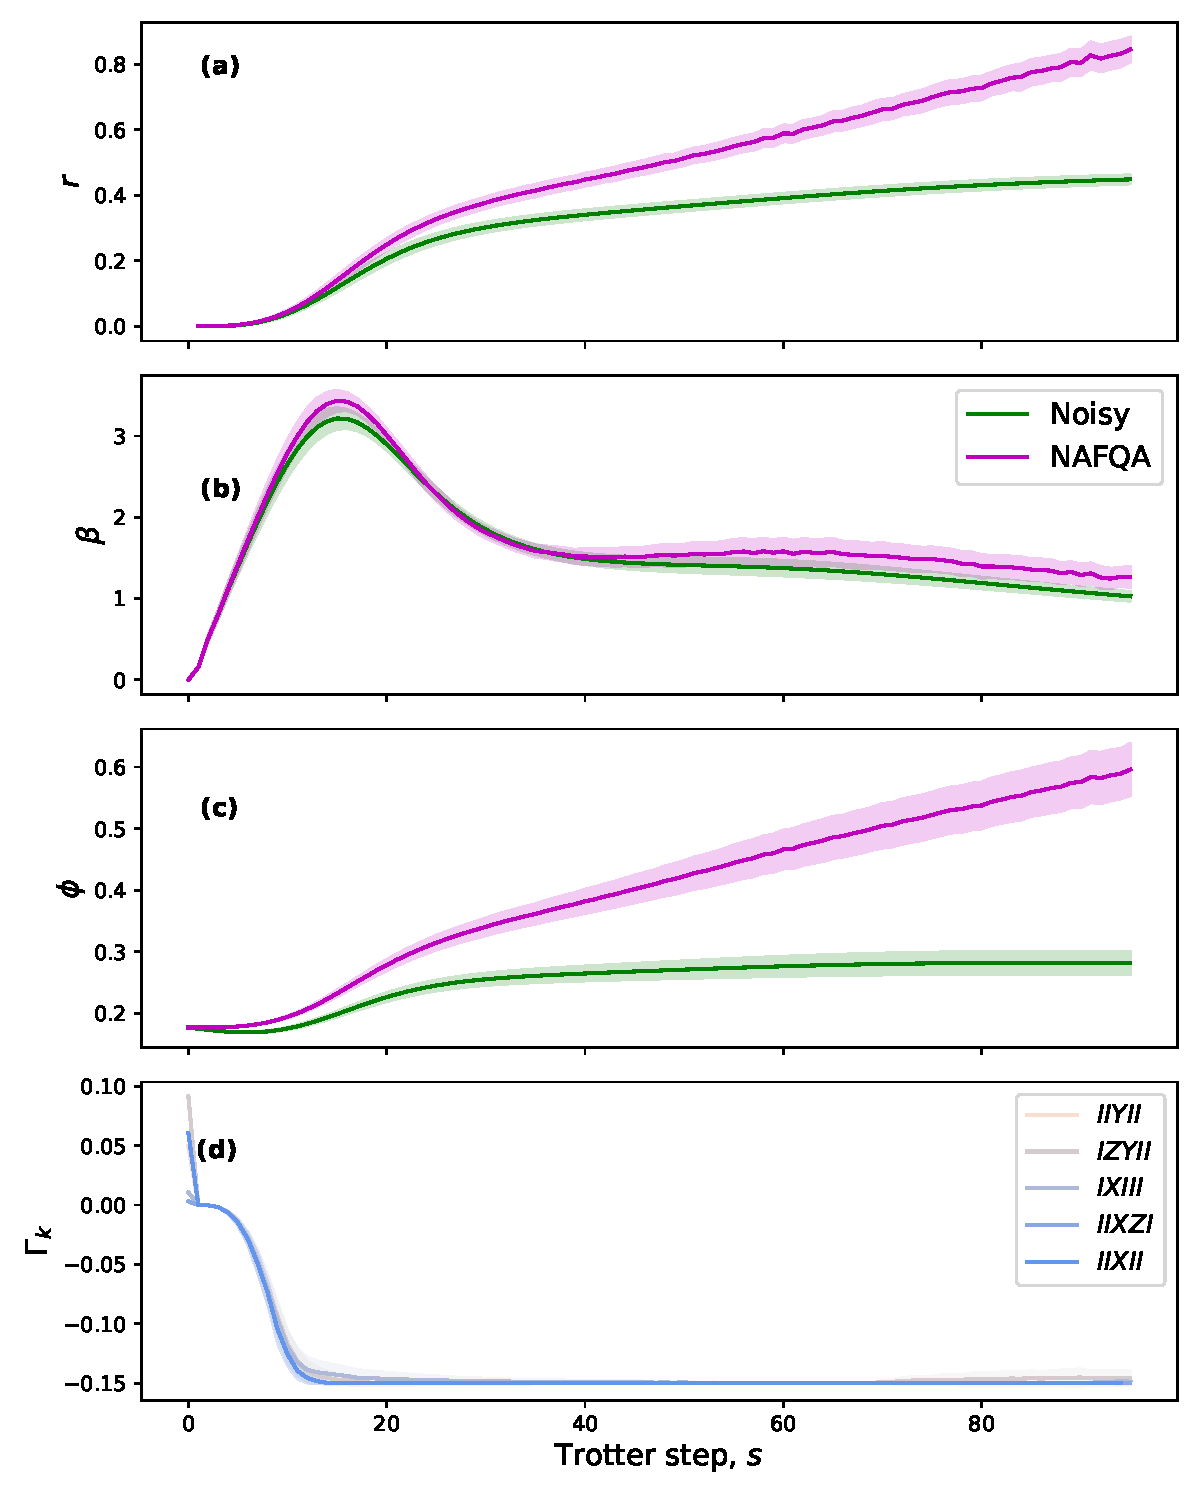
\includegraphics[scale=0.425]{final_plots/TFIM_N5.pdf} 
    \caption{The performance of NAFQA against the noisy FQA. The mean and standard error (a) approximation ratio $r$, (b) control field $\beta$, and (c) success probability $\phi$ for the {5-qubit} spin glass Hamiltonians over 25 instances (seeds 0 through 24) are illustrated. The numerical simulations are carried out with a time step of {$dt = 0.009$}, yielding NAFQA results from 5000 trajectories. (d) error probabilities $\Gamma_k(t)$ for {$k\in{IIYII, IZYII, IXIII, IIXZI, IIXII}$}.}\label{TFIM_plot}
\end{figure}

Because quantum systems are inherently open, it is both natural and advantageous to design control protocols and quantum algorithms grounded in OQS theory. At the same time, intrinsic device noise remains a major obstacle to quantum simulation. A crucial first step toward overcoming this challenge is to characterize the intrinsic noise relevant to a given algorithm, using techniques such as randomized benchmarking and error reconstruction. As environmental noise cannot be completely eliminated, developing algorithms that integrate and exploit the intrinsic noise of NISQ devices is highly desirable. In this work, we have established a noise-assisted quantum optimization framework and demonstrated its effectiveness on emulated IBM quantum processors. By combining a sparse learning protocol with the pseudo-Lindblad quantum trajectories or quasiprobabilistic decomposition approach, we simulated non-Markovian, time-dependent open quantum systems (OQS). Applying our algorithm to the MaxCut and spin-glass Hamiltonians, we achieved population transfer toward the virtual ground state. The simulation of negative rates incurs an exponential overhead with system size and requires extensive sampling and measurement statistics for efficient implementation. Future efforts to mitigate these limitations may form the basis for realizing quantum advantage.
  

\section*{Methods}
\subsection*{Learning the Pauli-Lindblad noise model}\label{Pauli_noise_learning}
Here, we provide an overview of the noise characterization process corresponding to the noise associated with each layer of a digital quantum circuit. The unitary evolution of quantum gates on current NISQ devices is hindered by noise and dissipation. The application of an ideal unitary $U$ on qubits makes the evolution $\mathcal{U}(\rho) = U\rho U^{\dagger}$. Since quantum gates are noisy, a noisy channel can be defined as the composition of the ideal unitary $U$ and noisy operation $\tilde{\Lambda}$, that is, $\mathcal{\tilde{U}} = U \circ \tilde{\Lambda}$. The Pauli twirling simplifies the noise model $\tilde{\Lambda}$, and converts any arbitrary noise on the quantum hardware into stochastic Pauli channels~\cite{Flammia2020}, as illustrated in Fig.~\ref{Fig: twilring_plot}. It is obtained by sampling random instances of Pauli operators around the noisy layers. Algebraically, this is expressed as
\begin{equation}
    \Lambda(\cdot) = \mathbb{E}_i \left[ P_i^\dagger \tilde{\Lambda} \left( P_i \cdot P_i^\dagger \right) P_i \right].\label{noise_map}
\end{equation}
For the dissipator considered in Eq.~\eqref{pauli_channel}, it is shown that the sparse Pauli Lindblad noise channel can be expressed as~\cite{vandenBerg2023_natphys}
\begin{equation}
    \Lambda(\rho) = \prod_{k\in\mathcal{K}} \left( \omega_k \cdot + (1-\omega_k) P_k \cdot P_k^{\dagger} \right) \rho, \label{noise_channel_Lambda}
\end{equation}
where $\omega_k = (1+e^{-2\lambda_k})/2$ and the error probabilities $\{\lambda\}$ characterize the intrinsic noise of the quantum hardware. For a detailed exposition of the sparse Pauli learning process, we refer the reader to~\cite{vandenBerg2023_natphys, Ferracin2024efficiently}.

\subsection*{Pseudo-Lindblad quantum trajectory unraveling}\label{PLQT}
Here, we present the PLQT approach~\cite{Eckardt_PRL} and discuss how it can be implemented in a digital quantum circuit to simulate non-Markovian dynamics. 

The simulation of a GKSL master equation requires the evolution of a density matrix $\rho$ of size $d_H^2$ when the Hilbert space has dimension $d_H$. However, simulating a state (wavefunction) instead of $\rho$ is numerically more efficient, since the state has dimension $d_H$. Therefore, the MCWF method was proposed as an alternative approach to simulate a master equation, taking an ensemble average over multiple trajectories~\cite{Dalibard_etal_prl, Carmichael1993Open}. After a time step $dt$, the state either evolves under the effective Hamiltonian $H_{\text{eff}}$ as
\begin{equation}
    \ket{\psi(t + dt )} \propto (1-i dt H_{\text{eff}}) \ket{\psi(t)} \label{det_evol},
\end{equation}
with probability $1 - \sum_k r_k(t) dt $, or a quantum jump occurs with probability $r_k(t) = || L_k \ket{\psi(t)} || ^ 2 / || \ket{\psi(t)} || ^ 2$ and the state evolves as
\begin{equation}
    \ket{\psi(t + dt )} \propto L_k \ket{\psi(t)}.\label{jump_evol}
\end{equation}
Here, the effective non-Hermitian Hamiltonian is $H_{\text{eff}} = H - \frac{i}{2} \sum_k L_k^{\dagger} L_k$. The stochastic Schr\"odinger equation for this unraveling can be expressed in the It\^{o} formalism as  \begin{equation}
    \ket{d\psi} = \sum_k dN_k \left( \frac{~~L_k}{\sqrt{r_k(t)}} \ket{\psi} - \ket{\psi} \right) + dt \left( \sum_k \frac{r_k(t)}{2} - i  H_{\text{eff}}\right) \ket{\psi}.
\end{equation}
$dN_k$ represents independent jump processes, with $dN_k$ being one (zero) in the event of a quantum jump (no quantum jump). 

The GKSL equation states that if $\mathcal{L}$ is the Liouvillian governing the OQS evolution according to the master equation $d\rho / dt = \mathcal{L} (\rho) $, then there exists a CPTP quantum channel of the form $\mathcal{E} (\rho) = \text{exp}(\mathcal{L}t)$ for the evolution of $\rho$. The noisy gates in a quantum circuit can be simulated with this quantum trajectory approach by writing a CPTP channel with the Kraus representation as 
\begin{equation}
    \mathcal{E} (\rho) = \sum_k M_k (dt) \rho M_k ^{\dagger} (dt),
\end{equation}
where $\sum_k M_k(dt) M_k ^{\dagger} (dt) = I$. This map can be implemented in a quantum circuit as a stochastic map, where the state is updated to $\ket{\psi'} = \frac{1}{\sqrt{r_k}} M_k(dt) \ket{\psi}$ with probability $r_k = |\braket{{\psi} | M_k ^{\dagger}(dt) M_k(dt) | {\psi}}|^2$. The Kraus operators representing Eqs.~\eqref{det_evol} and \eqref{jump_evol} for a Trotter step of $d t $ are given by 
\begin{equation}
    M_0(dt) = I -i H_{\text{eff}} dt ~ , ~ M_k(dt) = \sqrt{dt} L_k~, ~ k\neq0.
\end{equation}

\begin{figure}[t!]
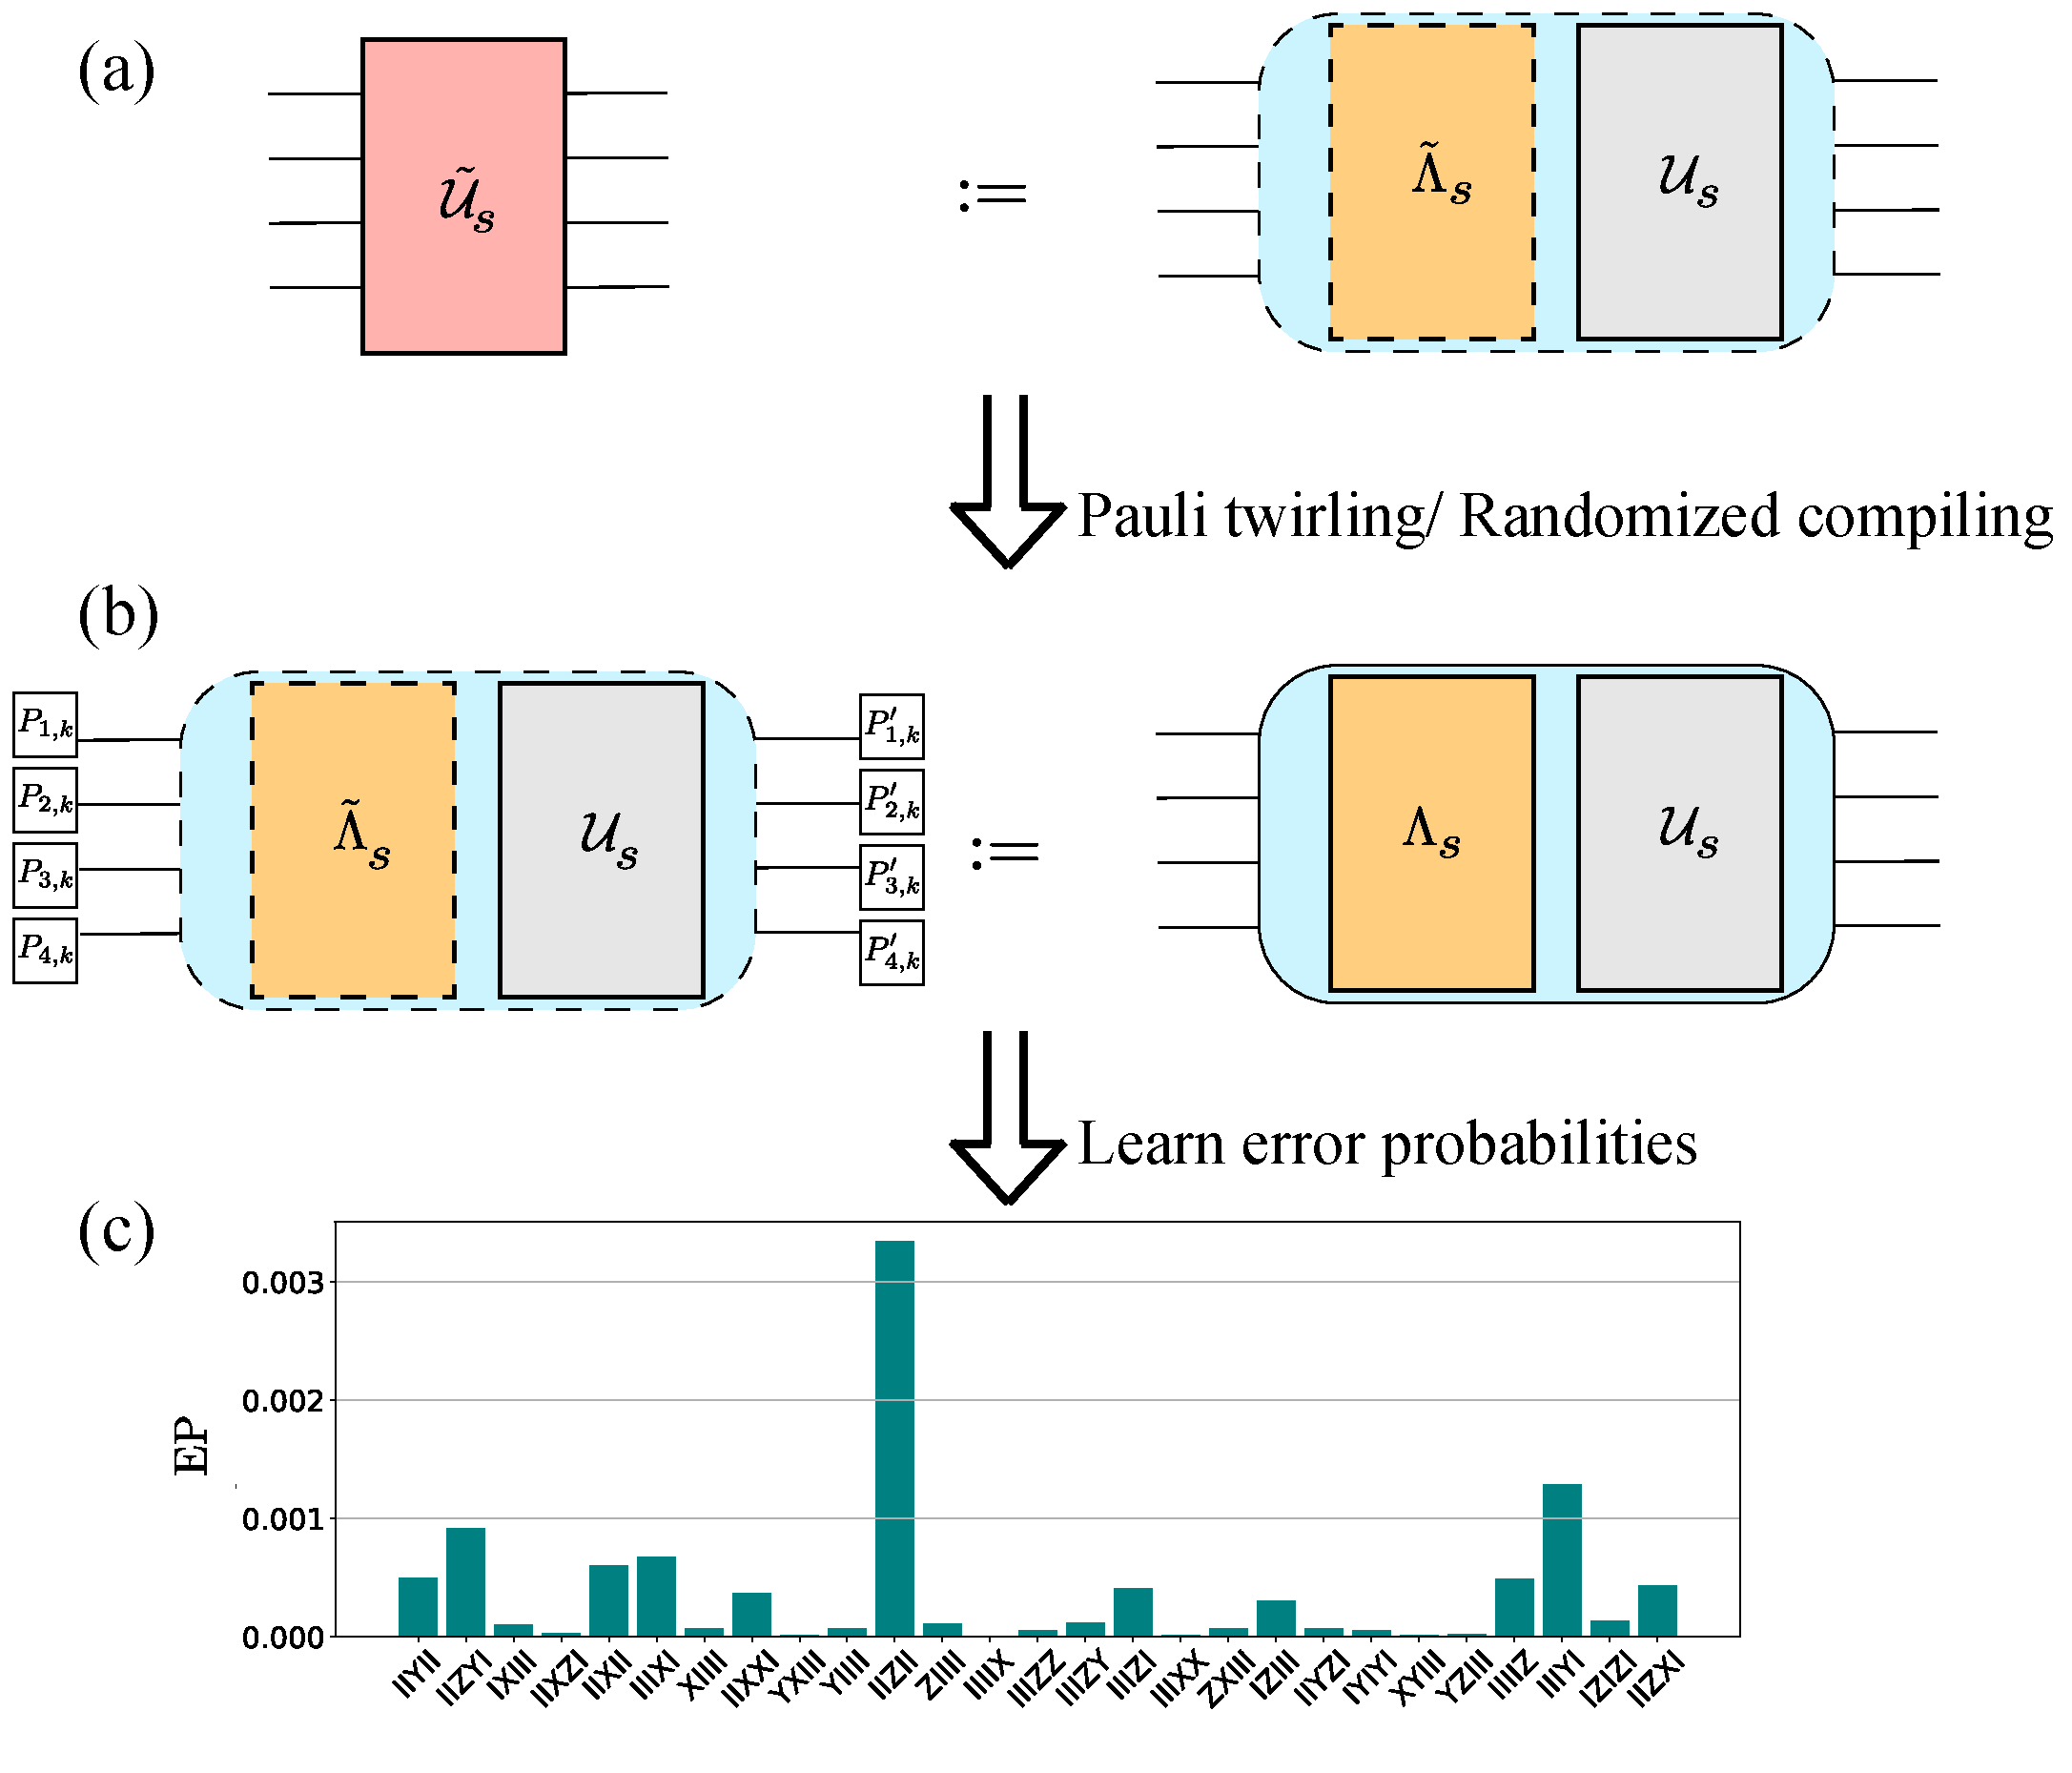
\includegraphics[scale=0.24]{final_plots/Learnerror.pdf} 
    \caption{\textbf{Overview of the noise modeling and learning.} (a) Ideal unitary at the $s^{\text{th}}$ layer whose action is denoted by $\mathcal{U}_s$ and its implementation on NISQ is $\tilde{\mathcal{U}}_s$, decomposed as $\tilde{\mathcal{U}}_s = \mathcal{U}_s \circ \tilde{\Lambda}_s$. (b) Pauli twirling or randomized compiling maps the noise channel $\tilde{\Lambda}_s$ to an effective stochastic Pauli channel ${\Lambda}_s$ by randomly applying one-qubit Pauli operators before and after the noisy layer. For Clifford operators $U$, we obtain $ P'_{n,s} = UP_{n,s}U^{\dagger}$, where $n$ is the $n^{\text{th}}$ qubit. (c) Learned error probabilities of the 5-qubit emulated IBM-Vigo simulator.
    } \label{Fig: twilring_plot}
\end{figure}
% Utilizing this noise map,
We extend this formalism to simulate layer-dependent non-Markovian dynamics on a digital quantum computer with the PLQT approach. It relies on extending the Hilbert space of the system by an additional classical bit $s \in \{-1, +1\}$. Since we are interested in the negative decay rates in the GKSL equation, Eq.~\eqref{na--qlc} can be modified as 
\begin{equation}
    \frac{d \rho}{dt} = -i [H, \rho] + \sum_k s_k (L_k \rho L_k^\dagger - \frac{1}{2} L_k^\dagger L_k \rho - \frac{1}{2} \rho L_k^\dagger L_k ),
\end{equation}
where each Lindblad operator $L_k$ is associated with a stochastic Pauli channel. This involves a positive relaxation strength $|\Gamma_k|$, as $L_k = \sqrt{|\Gamma_k|} P_k$. The signs $s_k = \Gamma_k / |\Gamma_k| = \pm 1$ are multiplied in the classical post-processing step to simulate the non-Markovian dynamics. In the It\^{o} formalism, the stochastic Schr\"odinger equation is described as 
\begin{equation}
    \ket{d\psi} = \sum_k dN_k \left( \frac{~s_k L_k}{\sqrt{r_k(t)}} \ket{\psi} - \ket{\psi} \right) + dt \left( \sum_k \frac{r_k(t)}{2} - i  H_{\text{eff}}'\right) \ket{\psi}, 
\end{equation}
where $H_{\text{eff}}' = H - \frac{i}{2} \sum_k s_k L_k^{\dagger} L_k$. As we are only concerned with modifying the noise channel, we do not consider the contribution of the unitary part that comes from the Hamiltonian $H$. Furthermore, for the Pauli noise channels considered in Eq.~\eqref{pauli_channel}, we have $\sum_k L_k^\dagger L_k \propto I$. Therefore, the non-Hermitian effective Hamiltonian becomes $H_{\text{eff}} = - \frac{i}{2} \sum_k s_k |\Gamma_k| I $, which introduces a global phase factor and can be ignored. The state undergoes a quantum jump 
\begin{equation}
\begin{split}
    \ket{\psi^{(k)}(t + dt)} & = \frac{\sqrt{|\Gamma_k|}P_k \ket{\psi(t)}}{\sqrt{r_k(t)}}, 
    s^{(k)}(t + dt) & = \frac{\Gamma_k}{|\Gamma_k|} s^{(k)}(t),
\end{split}
\end{equation}
with probability $r_k(t) dt$ and the identity operator $I$ acts with the remaining probability. The final-state density operator after evolution is obtained as $\rho(t) = \overline{s(t)\ket{\psi(t)}\bra{\psi(t)}}$. For the choice of Lindblad operators, we have $r_k = {|\Gamma_k|}$, which cancels out in the ensemble average. For a finite sample size $M$, the state at time $t$ can be renormalized as $\rho_{{M}}(t) = \frac{1}{\mathcal{N}} \sum_m^{{M}} s_m \ket{\psi_m(t) } \bra{\psi_m(t) }$, where $\mathcal{N} = \sum_k^{{M}} s_m \braket{\psi_m(t) | \psi_m(t)}$. Here, the Kraus operators can be written as a mixed unitary channel with $M_0 \propto I$ and $M_k \propto P_k$. 

{The sampling overhead of the PLQT method is intimately connected to that of the QPD approach. The average sign of the trajectory ensemble 
satisfies~\cite{Eckardt_PRL}
%
\begin{equation}
    \bar{s}(T) 
    = \exp\!\left[-2\sum_{k\in\mathcal{K}}
    \int_0^T|\nu_k(t)|\,dt\right]
    = \mathcal{N}(T)^{-1},
    \label{eq:sign_correspondence}
\end{equation}
%
where $\mathcal{N}(T)$ is the QPD sampling overhead of 
Eq.~(\ref{error_mitigation_cost}). The number of trajectories required to maintain a fixed precision, therefore, scales as $M \propto 1/\bar{s}(T)^2 = \mathcal{N}^2$, identical to the QPD cost. Both methods thus pay the same fundamental exponential overhead. This exponential cost is not an artifact of our implementation, but is fundamental in nature, bearing a direct structural analogy to the fermionic sign problem in quantum Monte Carlo simulations~\cite{Troyer_prl_2005}. Since Troyer and Wiese established that the sign problem is NP-hard~\cite{Troyer_prl_2005}, this analogy suggests that the exponential overhead for simulating negative Lindblad rates is likewise a fundamental barrier. We note that this analogy is structural and not a formal complexity-theoretic reduction.}

\subsection*{Quasiprobability decomposition for the experimental implementation}
The noise map $\Lambda'(\rho)$ corresponding to the Liouvillian $\mathcal{L}(\rho) = \sum_{k\in \mathcal{K}} s_k |\nu_k| (P_k \rho P_k^{\dagger} - \rho)$  can be simplified to~\cite{vandenBerg2023_natphys} 
\begin{equation}
    \Lambda'(\rho) = \prod_{k\in\mathcal{K}} \left( \omega'_k \cdot + s_k (1-\omega'_k) P_k \cdot P_k^{\dagger} \right) \rho,
\end{equation}
where $\omega'_k = (1+e^{-2 |\nu_k| })/2$, and the sampling overhead $\mathcal{N} = \omega'_k +  s_k (1-\omega'_k)$  is consistent with Eq.~\eqref{samp_over}. The sampling algorithm to virtually implement the $\Lambda'$ is as follows:
\begin{enumerate}
    \item For every $k\in\mathcal{K}$, sample the identity matrix with probability $\omega'_k$, and the Pauli matrix $P_k$ with probability $1-\omega'_k$.
    \item Store the sign $s_k$ when the Pauli matrix is sampled. 
    \item Measure the expectation value for each sampling at the end of the circuit (executed on a quantum computer) and multiply its sign (on a classical computer).
    \item Measure the final expectation value after sampling over all the estimators and finally scale it with the sampling overhead $\mathcal{N}$ (on a classical computer), as given in Eq.~\eqref{qpd_eqn}.
\end{enumerate}

The targeted coefficients $\Gamma_k(t)$ in Eq.~\eqref{na--qlc} for each layer can be obtained by integrating the noise learning process with the QPD approach. Utilizing the property of channel operations, we have $\Gamma_k(t) = \lambda_k + \nu_k(t)$. Using $\{\nu_k(t)\}$ and $\{\lambda_k\}$ the modified stochastic noisy map $\mathcal{F}_s$ can be expressed as $\mathcal{F}_s = \Lambda_s \circ \Lambda_s'$, as given in Eq.~\eqref{non_Markovian-ckt}. Here, the subscript $s$ denotes the Trotter step $s$. The state of the system at time $t+dt$ is then given by 
\begin{equation}
    \rho(t+ dt) = \mathcal{{U}}_s \mathcal {F}_s (\rho(t)).
\end{equation}
Starting from an initial pure state $\rho_0$ at time $t = 0$, the final state after performing NAFQA for $s$ Trotter steps will be closer to the approximate virtual ground state of the system, i.e., $\rho(s ~dt)$ approaches the approximate virtual ground state.

\section*{Data Availability}
The data to reproduce all figures are available at the GitHub repository~\cite{nafqa_kasturi}.

\section*{Code Availability}
The code to reproduce all figures is available at the GitHub repository~\cite{nafqa_kasturi}.

\section*{Acknowledgements}
It is a pleasure to thank Peter Zoller for numerous insightful suggestions that helped improve the manuscript. KRS further thanks Kazutaka Takahashi, Pablo Martínez-Azcona, and András Grabarits for useful discussions. This research was funded by the Luxembourg National Research Fund (FNR),  via the FNR-CORE Grant ``AQCQNET'' (C22/MS/17132054). 

\section*{Author Contributions}
K.R.S. conceived the original idea and performed the numerical simulations. R.K.M. and A.d.C. contributed to further refining and developing the results. R.K.M. plotted the schematic diagrams. All authors contributed to the writing of the manuscript and the analysis of the results. All authors have read and approved the manuscript.

\section*{Competing Interests}
The authors declare no competing financial or non-financial interests. Author Rajesh K.\ Malla is an Associate Editor of Physical Review Letters. Rajesh K.\ Malla was not involved in the journal’s review of, or decisions related to, this manuscript.

\section*{References} 
\bibliography{reference.bib}
\\

\noindent \textbf{Correspondence} and requests for materials should be addressed to Kasturi Ranjan Swain.

\end{document}
